\chapter{Povezivanje razvojnog sustava i oblaka}

Oblak koju pruža platforma AWS i razvojni sustav ESP32-C3 dva su odvojena sustava koja moraju međusobno komunicirati i razmjenjivati podatke. Za ostvarenje njihove veze razvijena su dva programska rješenja:
\begin{enumerate}
	\item programska potpora za mikrokontroler, koja će omogućiti dinamičko povezivanje na Wi-Fi, spajanje na platformu AWS te slanje podataka u oblak,
	\item programska potpora za platformu AWS, koja će ostvariti umrežavanje uređaja u sustav, ažuriranje softvera na uređaju, pohranu primljenih podataka s uređaja te prikaz tih podataka u web aplikaciji. 
\end{enumerate} 

\section{Programska potpora za mikrokontroler}

Za razvoj programske potpore za mikrokontroler korišten je paket za razvoj softvera \textit{ESP-AWS-IoT} \engl{Software Development Kit - SDK} tvrtke \textit{Espressif}. To je repozitorij otvorenog koda temeljen na službenom programskom paketu tvrtke Amazon koji omogućava ugradbenim računalima razvijanih u programskom jeziku C komunikaciju s AWS-om. Korišteni razvojni paket omogućava uređajima temeljnim na ESP32 jezgri povezivanje sa uslugama platforme AWS. Pojednostavljuje integraciju uređaja s AWS ekosustavom nudeći gotova sučelja i programske primjere za sve značajke \cite{esp_aws_iot}. Razvijena programska potpora za uređaj ESP32-C3 sastoji se od nekoliko komponenti:
\begin{itemize}
	\item dinamičko povezivanje na bežičnu mrežu,
	\item spajanje na platformu AWS,
	\item učitavanje novog softvera, 
	\item očitavanje senzorskih mjerenja, 
	\item slanje podataka u oblak protokolom MQTT.
\end{itemize}

Neke od navedenih komponenti izvršavaju se slijedno, dok se druge izvršavaju paralelno. Spajanje na Wi-Fi i povezivanje s platformom AWS ključni su koraci koji prethode bilo kakvom pokušaju slanja podataka u oblak. Isto tako, praćenje ažuriranja softvera i očitavanje mjerenja izvršavaju se paralelno u posebnim procesima budući da nisu sekvencijalni niti međusobno isključivi zadaci. U nastavku je pobliže opisan svaki navedeni segment programske potpore. 

\subsection{Dinamičko povezivanje mikrokontrolera na Wi-Fi}

Radni okvir ESP-IDF nudi dinamičko spajanje na Wi-Fi mrežu pomoću zasebne komponente. Ovaj se postupak naziva provizioniranje \engl{provisioning}. Ova komponenta pruža aplikacijska programska sučelja \engl{Application Programming Interface - API} koja kontroliraju pružanje usluge za primanje i konfiguriranje Wi-Fi vjerodajnica putem sigurnih komunikacijskih protokola. Sigurnosni protokoli definirani su u komponenti protokolne komunikacije \engl{protocomm} koja upravlja sigurnim sjednicama \engl{sessions} i pruža radni okvir za višestruki prijenos podataka. Također je moguće direktno koristiti sloj protokolne komunikacije radi implementacije specifične za aplikaciju \cite{unified_provisioning}.

Sloj protokolne komunikacije interno koristi mehanizam protokolnih međuspremnika \engl{protocol buffers - protobuf} za sigurno uspostavljanje sjednice. Protokolni međuspremnici namijenjeni su za serijalizaciju strukturiranih podataka neovisno o programskom jeziku i platformi. Koristan je pri izradi programa i sustava koji međusobno komuniciraju putem mreže zbog kompaktnosti i niske latencije \cite{what_is_protobuf}.

Sloj protokolne komunikacije pruža radni okvir za različite načine komunikacije:
\begin{enumerate}
	\item protokol BLE,
	\item Wi-Fi (SoftAP u kombinaciji s HTTP serverom).
\end{enumerate}

Pružajući korisnicima okvir za ostvarivanje usluge dinamičkog povezivanja u mrežu, neovisno o načinu komunikacije, ovakva vrsta podrške naziva se unificirano provizioniranje \engl{unified provisioning}. Ovakav način prijave uređaja na mrežu zahtijeva interakciju korisnika putem vanjskog uređaja za slanje vjerodajnica na mikrokontroler. Tvrtka \textit{Espressif} pruža jednostavna mobilna rješenja koja se mogu koristiti gotova ili pak uklopiti u vlastitu mobilnu aplikaciju. Na slici \ref{fig:unified_provisioning} prikazana je arhitektura usluge.

\begin{figure}[ht]
	\centering
	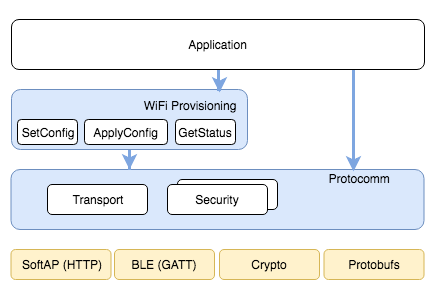
\includegraphics[scale=0.8]{imgs/unified_provisioning}
	\caption{Arhitektura unificiranog provizioniranja \cite{unified_provisioning}}
	\label{fig:unified_provisioning}
\end{figure}

Kao što je ranije opisano, arhitektura je bazirana na sloju protokolne komunikacije koji je odgovoran za prijenos podataka i sigurnost. Služi za jednostavne povratne pozive aplikaciji \engl{callbacks} i dobivanje Wi-Fi statusa. Sama aplikacija ima kontrolu nad implementacijom povratnih poziva. 

Aplikacija stvara instancu protokolne komunikacije koja se preslikava na određeni prijenosni protokol i sigurnosnu shemu. Svaki prijenos podataka u sloju protokolne komunikacije ima koncept krajnje točke \engl{endpoint} koji odgovara logičkom komunikacijskom kanalu za određenu vrstu informacija. Primjerice, sigurnosno rukovanje \engl{handshake} odvija se na različitoj krajnjoj točki u odnosu na točku za Wi-Fi konfiguraciju. Svaka se krajnja točka identificira nizom znakova i mijenja se ovisno o internom prikazu krajnje točke. U slučaju prijenosa pomoću Wi-Fi veze odnosno SoftAP funkcionalnosti, krajnja točka prikazuje se kao URI, dok u slučaju prijenosa podataka putem protokola BLE odgovara GATT karakteristici sa specifičnim identifikatorom. 

Oglašavanje i otkrivanje uređaja prepušteno je aplikaciji i ovisno o odabranom protokolu, vanjske aplikacije mogu odabrati odgovarajuću metodu za oglašavanje i otkrivanje. Za Wi-Fi prijenos obično se koristi ime mreže pristupne točke. Za prijenos putem protokola BLE može se koristiti ime samog uređaja. 

Kao što je opisano, podržano je korištenje protokola BLE kao i Wi-Fi usluge za prijenos vjerodajnica. Pri odabiru prijenosnog kanala za spajanje uređaja u mrežu, potrebno je razmotriti nekoliko točaka. Za početak, prijenos temeljen na protokolu BLE prednost održavanja netaknutog komunikacijskog kanala između uređaja i klijenta tijekom prijenosa podataka, što osigurava pouzdanu povratnu informaciju. S druge strane, prijenos putem Bluetootha troši oko 110 KB memorije tijekom rada, što je na uređajima niskih resursa velika potrošnja. Korisno je što se korištena memorija može vratiti na hrpu \engl{heap} po završetku umrežavanja uređaja ukoliko se BLE funkcionalnosti više ne koriste. Prijenos temeljen na Wi-Fi mreži, odnosno SoftAP funkcionalnosti, vrlo je interoperabilan i ne troši dodatnu memoriju. Međutim, mikrokontroler koristi isti radio za emitiranje pristupne točke i za spajanje na željenu mrežu. Budući da se te akcije mogu odvijati na različitim kanalima, postoji mogućnost da se ažuriranja statusa veze ne dostave na mobilni uređaj. Također, mobilni se uređaj mora odspojiti s izvorne Wi-Fi mreže radi privremenog spajanja na pristupnu točku mikrokontrolera. Uređaj će se spojiti na izvornu mrežu tak kada mikrokontroler ugasi pristupnu točku \cite{unified_provisioning}. 

Za razvoj predloženog rješenja korišteno je slanje vjerodajnica pomoću Wi-Fi mreže, odnosno privremene pristupne točke. Kao što je ranije opisano, protokol BLE troši značajnu količinu \textit{heap} memorije, a razvojni sustav ESP32-C3 nema dovoljno radne memorije koja bi pokrila prijavu u mrežu uz ostale radne procese. Mikrokontroler najprije stvori privremenu pristupnu točku na koju se mobilni uređaj spaja pomoću mobilne aplikacije. Zatim, nakon skeniranja dostupnih Wi-Fi mreža u blizini, u mobilnoj aplikaciji odabire se željena mreža i unese lozinka. Vjerodajnice se zatim pošalju putem Wi-Fi mreže, i mobilni uređaj može se odspojiti s privremene pristupne točke. Vjerodajnice se pohrane u memoriju tipa NVS \engl{non-volatile storage} koja ne zahtijeva konstantno napajanje kako bi se zadržala na uređaju. Ovime je omogućeno povezivanje uređaja u sustav čak i kada dođe do prekida napajanja \cite{what_is_nvs}. Memorija tipa NVS može se jedino programski obrisati, te bi u idealnom izvedbenom rješenju postojao vanjski gumb spojen na mikrokontroler koji bi pokretao brisanje te memorije i tako omogućio ponovno spajanje na željenu mrežu. Sljedeći programski isječak prikazuje inicijalizaciju memorije NVS, mrežnog sučelja te stvaranje pristupne točke.

\begin{lstlisting}[caption={Stvaranje pristupne točke}, language=c]
	/* Init NVS partition */
	esp_err_t ret = nvs_flash_init();
	/* Init TCP/IP */
	ESP_ERROR_CHECK(esp_netif_init());
	/* Init the event loop */
	ESP_ERROR_CHECK(esp_event_loop_create_default());
	wifi_event_group = xEventGroupCreate();
	/* Init Wi-Fi including netif with default config */
	esp_netif_create_default_wifi_sta();
	esp_netif_create_default_wifi_ap();
	wifi_prov_mgr_config_t config = {
		.scheme = wifi_prov_scheme_softap,
		.scheme_event_handler = WIFI_PROV_EVENT_HANDLER_NONE
	};
    /* Init provisioning manager with above config */
	ESP_ERROR_CHECK(wifi_prov_mgr_init(config));
	ESP_ERROR_CHECK(wifi_prov_mgr_start_provisioning(security, (const void *) sec_params, service_name, service_key));
	wifi_prov_print_qr(service_name, username, pop, PROV_TRANSPORT_SOFTAP, disp);
\end{lstlisting}

\subsubsection{LCD zaslon}

Za povezivanje mobilnog uređaja na privremenu pristupnu točku koju emitira razvojni sustav, potrebno je skenirati QR kod koji mikrokontroler generira. Budući da ESP32-C3 nema vlastito sučelje, na sustav je spojen zaslon OLED SSD1306 veličine 128×64 piksela. Uređaj sa zaslonom komunicira putem I2C sučelja, a za prikaz sadržaja na zaslonu korištena je biblioteka LVGL \engl{Light and Versatile Graphics Library}. To je grafička biblioteka otvorenog koda namijenjena izradi aplikacija s grafičkim korisničkim sučeljem \engl{Graphical User Interface - GUI} za ugradbene sustave. Pruža radni okvir s mnogim značajkama, temama i paletama boja. Isto tako, biblioteka troši vrlo malo resursa, što je čini pogodnom za uređaje poput razvojnog sustava ESP32-C3 \cite{lvgl}. Generiranje QR koda obavlja se pomoću biblioteke \textit{QR-Code-Generator} koja je prilagođena ESP32 uređajima. Tablica \ref{table:pinout_lcd} prikazuje način spajanja pločice sa zaslonom. Kao što se vidi iz konfiguracije, osim napajanja i uzemljenja, potrebno je spojiti liniju za prijenos podataka te liniju takta. 

\begin{table}[ht!]
	\centering
	\caption{Povezivanje uređaja i LCD zaslona}
	\begin{tabular}{|c| c|}
		\hline
		\rowcolor{lightblue}  
		\textbf{Pin razvojnog sustava} & \textbf{Pin zaslona} \\ \hline
		GND & GND \\ \hline
		5V & Vcc \\ \hline
		GPIO 4 & SCL  \\ \hline
		GPIO 5 & SDA \\ \hline
	\end{tabular}
	\label{table:pinout_lcd}
\end{table}

\begin{lstlisting}[caption={Generiranje QR koda iz pristupne točke}, language=c]
static void wifi_prov_print_qr(const char *name, const char *usrname, const char *pop, const char *transport, lv_disp_t *disp) {
	char payload[150] = {0};
    snprintf(payload, sizeof(payload), 	
    	"{\"ver\":\"%s\",\"name\":\"%s\",\"username\":\"%s\",\"pop\":\"%s\",\"transport\":\"%s\"}",
    	 PROV_QR_VERSION, name, usrname, pop, transport);
    esp_qrcode_config_t cfg = {
		.display_func = generate_qr_code_lcd, 
		.max_qrcode_version = 10, 
		.qrcode_ecc_level = ESP_QRCODE_ECC_LOW
	};
	esp_qrcode_generate(&cfg, payload);
}
\end{lstlisting}

Prethodna funkcija povezuje pristupnu točku s QR kodom. Podaci o samoj pristupnoj točki učitaju se u privremenu varijablu, čiji se sadržaj prosljeđuje biblioteci za generiranje QR koda. Dobiveni se podaci zatim prosljeđuju funkciji za prikaz koda na zaslonu. QR kod prikazuje se na zaslonu piksel po piksel, skalirajući veličinu QR koda na temelju širine i duljine samog zaslona. 

\begin{lstlisting}[caption={Funkcija za prikaz QR koda na zaslonu}, language=c]
void generate_qr_code_lcd(esp_qrcode_handle_t qrcode)
{
	ESP_LOGI(TAG, "%s", "Started generate_qr_code_lcd...");
	
	int size = qrcodegen_getSize(qrcode);
	
	// Calculate the scale factor
	int scale = (int)fmin(EXAMPLE_LCD_H_RES / size, EXAMPLE_LCD_V_RES / size);
	
	// Calculate horizontal shift
	int shift_x = (EXAMPLE_LCD_H_RES - size * scale)/2;
	
	// Calculate vertical shift
	int shift_y = (EXAMPLE_LCD_V_RES - size * scale)/2;
	
	if (lvgl_port_lock(0)) {
		lv_obj_t *screen = lv_scr_act();
		lv_obj_clean(screen); // Clear the screen to ensure it's dark
		
		// Create a canvas object
		lv_obj_t *canvas = lv_canvas_create(screen);
		static lv_color_t cbuf[LV_CANVAS_BUF_SIZE_TRUE_COLOR(EXAMPLE_LCD_H_RES, EXAMPLE_LCD_V_RES)];
		lv_canvas_set_buffer(canvas, cbuf, EXAMPLE_LCD_H_RES, EXAMPLE_LCD_V_RES, LV_IMG_CF_TRUE_COLOR);
		lv_canvas_fill_bg(canvas, lv_color_white(), LV_OPA_COVER);
		
		// Draw the QR code on the canvas
		for (uint8_t y = 0; y < size; y++) {
			for (uint8_t x = 0; x < size; x++) {
				if (qrcodegen_getModule(qrcode, x, y)) {
					for (int dy = 0; dy < scale; dy++) {
						for (int dx = 0; dx < scale; dx++) {
							lv_canvas_set_px(canvas, shift_x + x * scale + dx, shift_y + y * scale + dy, lv_color_black());
						}
					}
				}
			}
		}
		
		// Release the mutex
		lvgl_port_unlock();
	}
}
\end{lstlisting}

Na slikama \ref{fig:esp_softap_app1} i \ref{fig:esp_softap_app2} prikazana je mobilna aplikacija te trenutak nakon skeniranja QR koda. Mobilni uređaj zahtijeva spajanje na privremenu pristupnu točku, a iduća slika prikazuje dostupne Wi-Fi mreže u blizini mobilnog uređaja, ujedno i mikrokontrolera, na koje se razvojni sustav može spojiti. Odabirom jedne od mreža i unosom lozinke vjerodajnice se šalju na razvojni sustav.

\begin{figure}[ht]
	\begin{minipage}[t]{0.3\textwidth}
		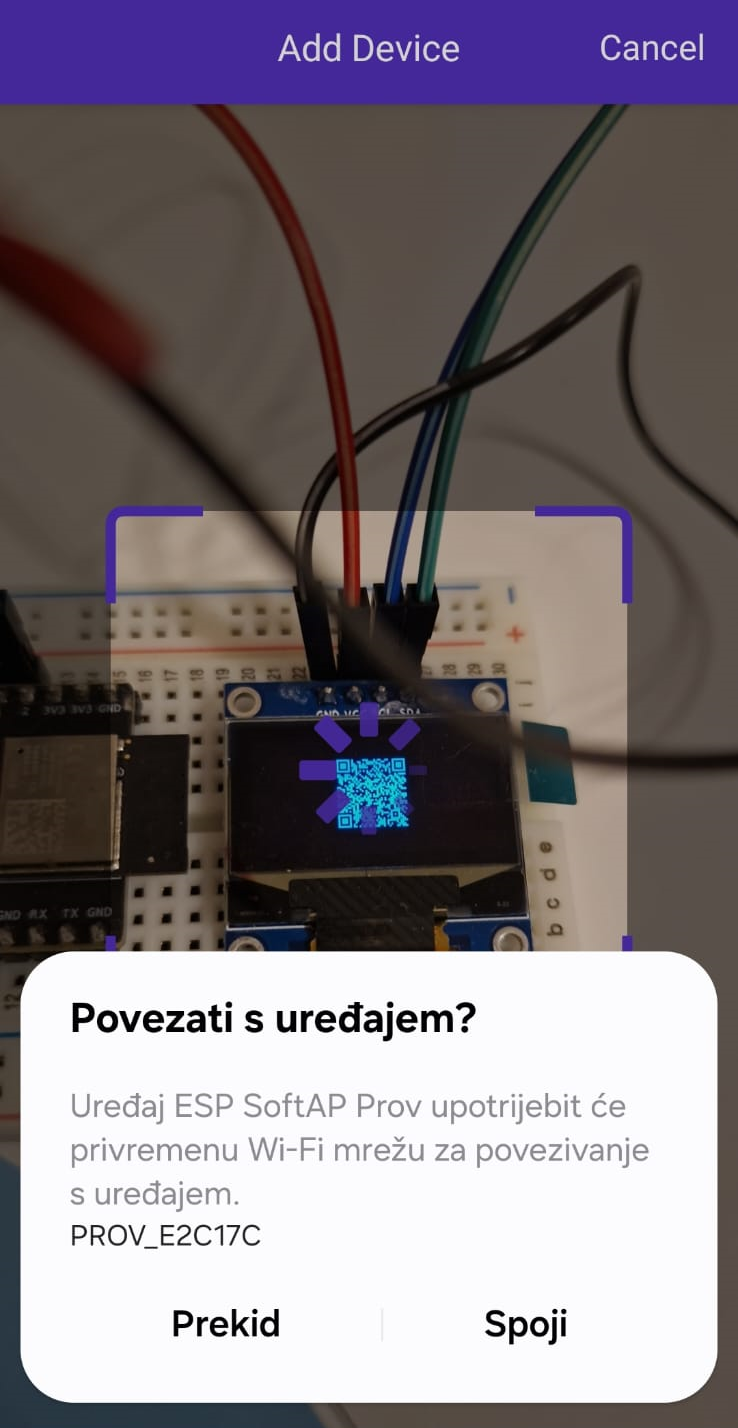
\includegraphics[width=\linewidth]{imgs/esp_softap_app1}
		\caption{Obavijest nakon skeniranja QR koda}
		\label{fig:esp_softap_app1}
	\end{minipage}
	\hspace*{\fill}
	\begin{minipage}[t]{0.3\textwidth}
		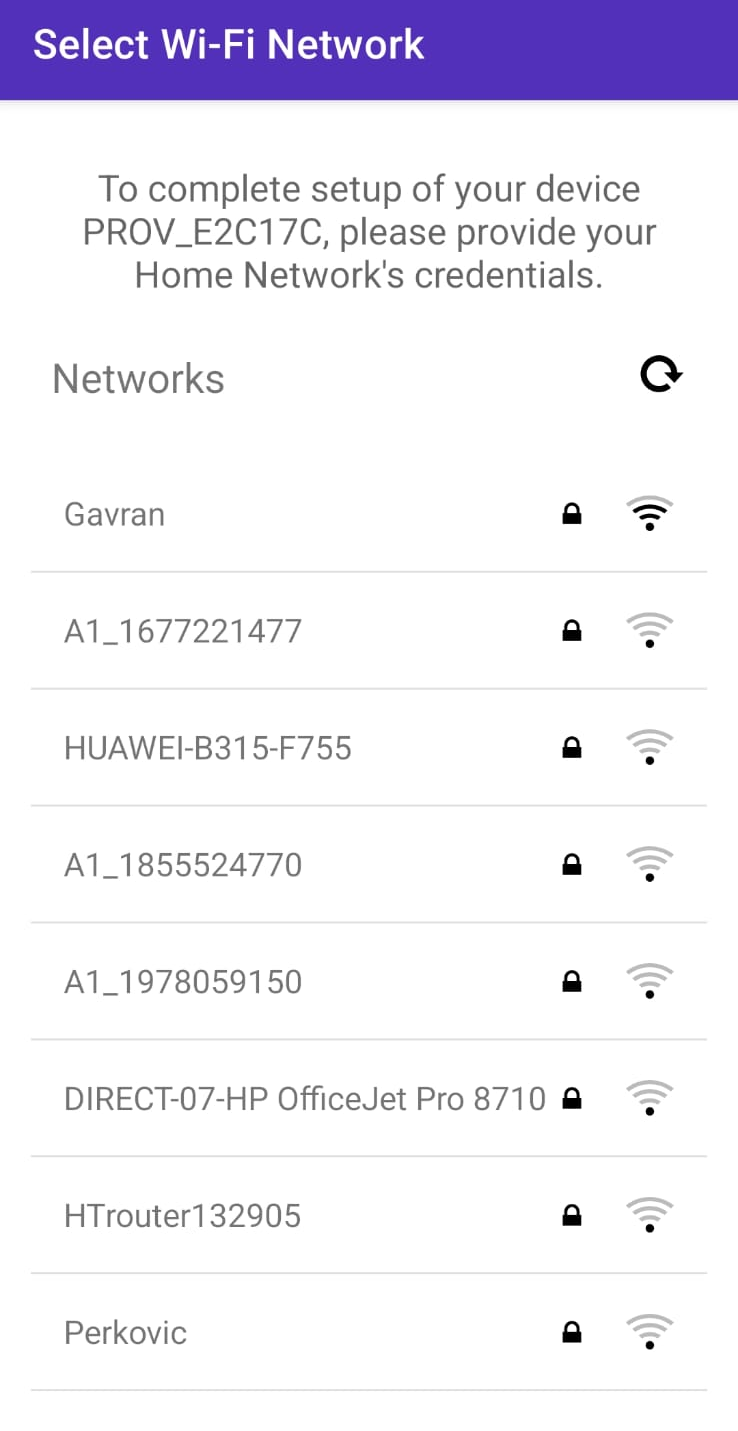
\includegraphics[width=\linewidth]{imgs/esp_softap_app2}
		\caption{Odabir dostupne Wi-Fi mreže u blizini}
		\label{fig:esp_softap_app2}
	\end{minipage}
\end{figure}

\subsection{Registracija u sustav AWS}

Nakon uspješnog povezivanja na Wi-Fi, sljedeći je korak registracija uređaja na platformu AWS. Korištena je biblioteka za AWS IoT Fleet Provisioning koja se održava u sklopu projekta otvorenog koda \textit{FreeRTOS} \cite{fleet_prov_sdk}. Biblioteka omogućuje mnoštvu odn. floti IoT uređaja registraciju i instalaciju jedinstvenih certifikata na platformu. Bibliotekom je moguće uređaje registrirati i pomoću autoriziranog korisnika, ali i certifikatima zahtjeva. Ova biblioteka ne ovisi o dodatnim bibliotekama osim standardne C biblioteke i stoga se može koristiti s bilo kojom bibliotekom za MQTT protokol.

Za potrebe ovog sustava odabrana je registracija pomoću certifikata zahtjeva. Na slici \ref{fig:fleet_provisioning_by_claim} prikazan je slijed događaja pri registraciji uređaja. Uređaj se najprije spaja na AWS certifikatom zahtjeva koji unaprijed postoji na mikrokontroleru te ostvaruje MQTT vezu. Zatim objavljuje praznu poruku na temu \textit{\$aws/certificates/create/json}, kojom zapravo podnosi zahtjev za kreiranjem vlastitog jedinstvenog certifikata. Usluga kreira traženi certifikat, pripadni ključ te generira značku vlasništva \engl{ownership token}, što sve skupa i objavljuje na temu \textit{\$aws/certificates/created/json/accepted}, na koju je uređaj pretplaćen. Razvojni sustav zatim sigurno pohranjuje dobivene vjerodajnice te objavljuje vlastite parametre i dobivenu značku na temu predloška za registraciju. Ako je kreirana, u sustavu AWS zatim se pokreće Lambda funkcija koja obavlja dodatne provjere nad dobivenim parametrima i tako provjerava valjanost zahtjeva. Primjerice, uređaj pri slanju parametara šalje i hardversku tajnu, koja se može zatim provjeriti u bazi podataka sustava AWS s pohranjenim takvim tajnama i provjeriti valjanost te tajne. Pri uspješnoj provjeri, Lambda funkcija vraća \lstinline|{"allowProvisioning" : True}|, čime daje konačno zeleno svjetlo za registraciju. Usluga posljedično kreira stvar i pripadnu politiku definiranu u predlošku te aktivira novostvoreni certifikat. Objavljuje novu konfiguraciju specifičnu za uređaj na temu za potvrdu uspješne registracije. Razvojni se sustav, nakon primjene nove konfiguracije, povezuje jedinstvenim privatnim ključem te certifikatom na AWS. Ova se nova MQTT veza dalje koristi za komunikaciju i razmjenu podataka. Ako je prvotno povezivanje neuspješno, aplikacija pokušava spojiti uređaj još dva puta prije nego se spajanje smatra potpuno neuspjelim. U tom slučaju, daljnje akcije čitanja mjerenja i slanja u oblak ne pokreću se jer je spajanje na platformu ključno za ostale radnje, stoga aplikacija izlazi iz glavnog programa. Jedino se ponovnim pokretanjem sustav može ponovno pokušati spojiti na internet i na platformu. 

\begin{figure}[ht]
	\centering
	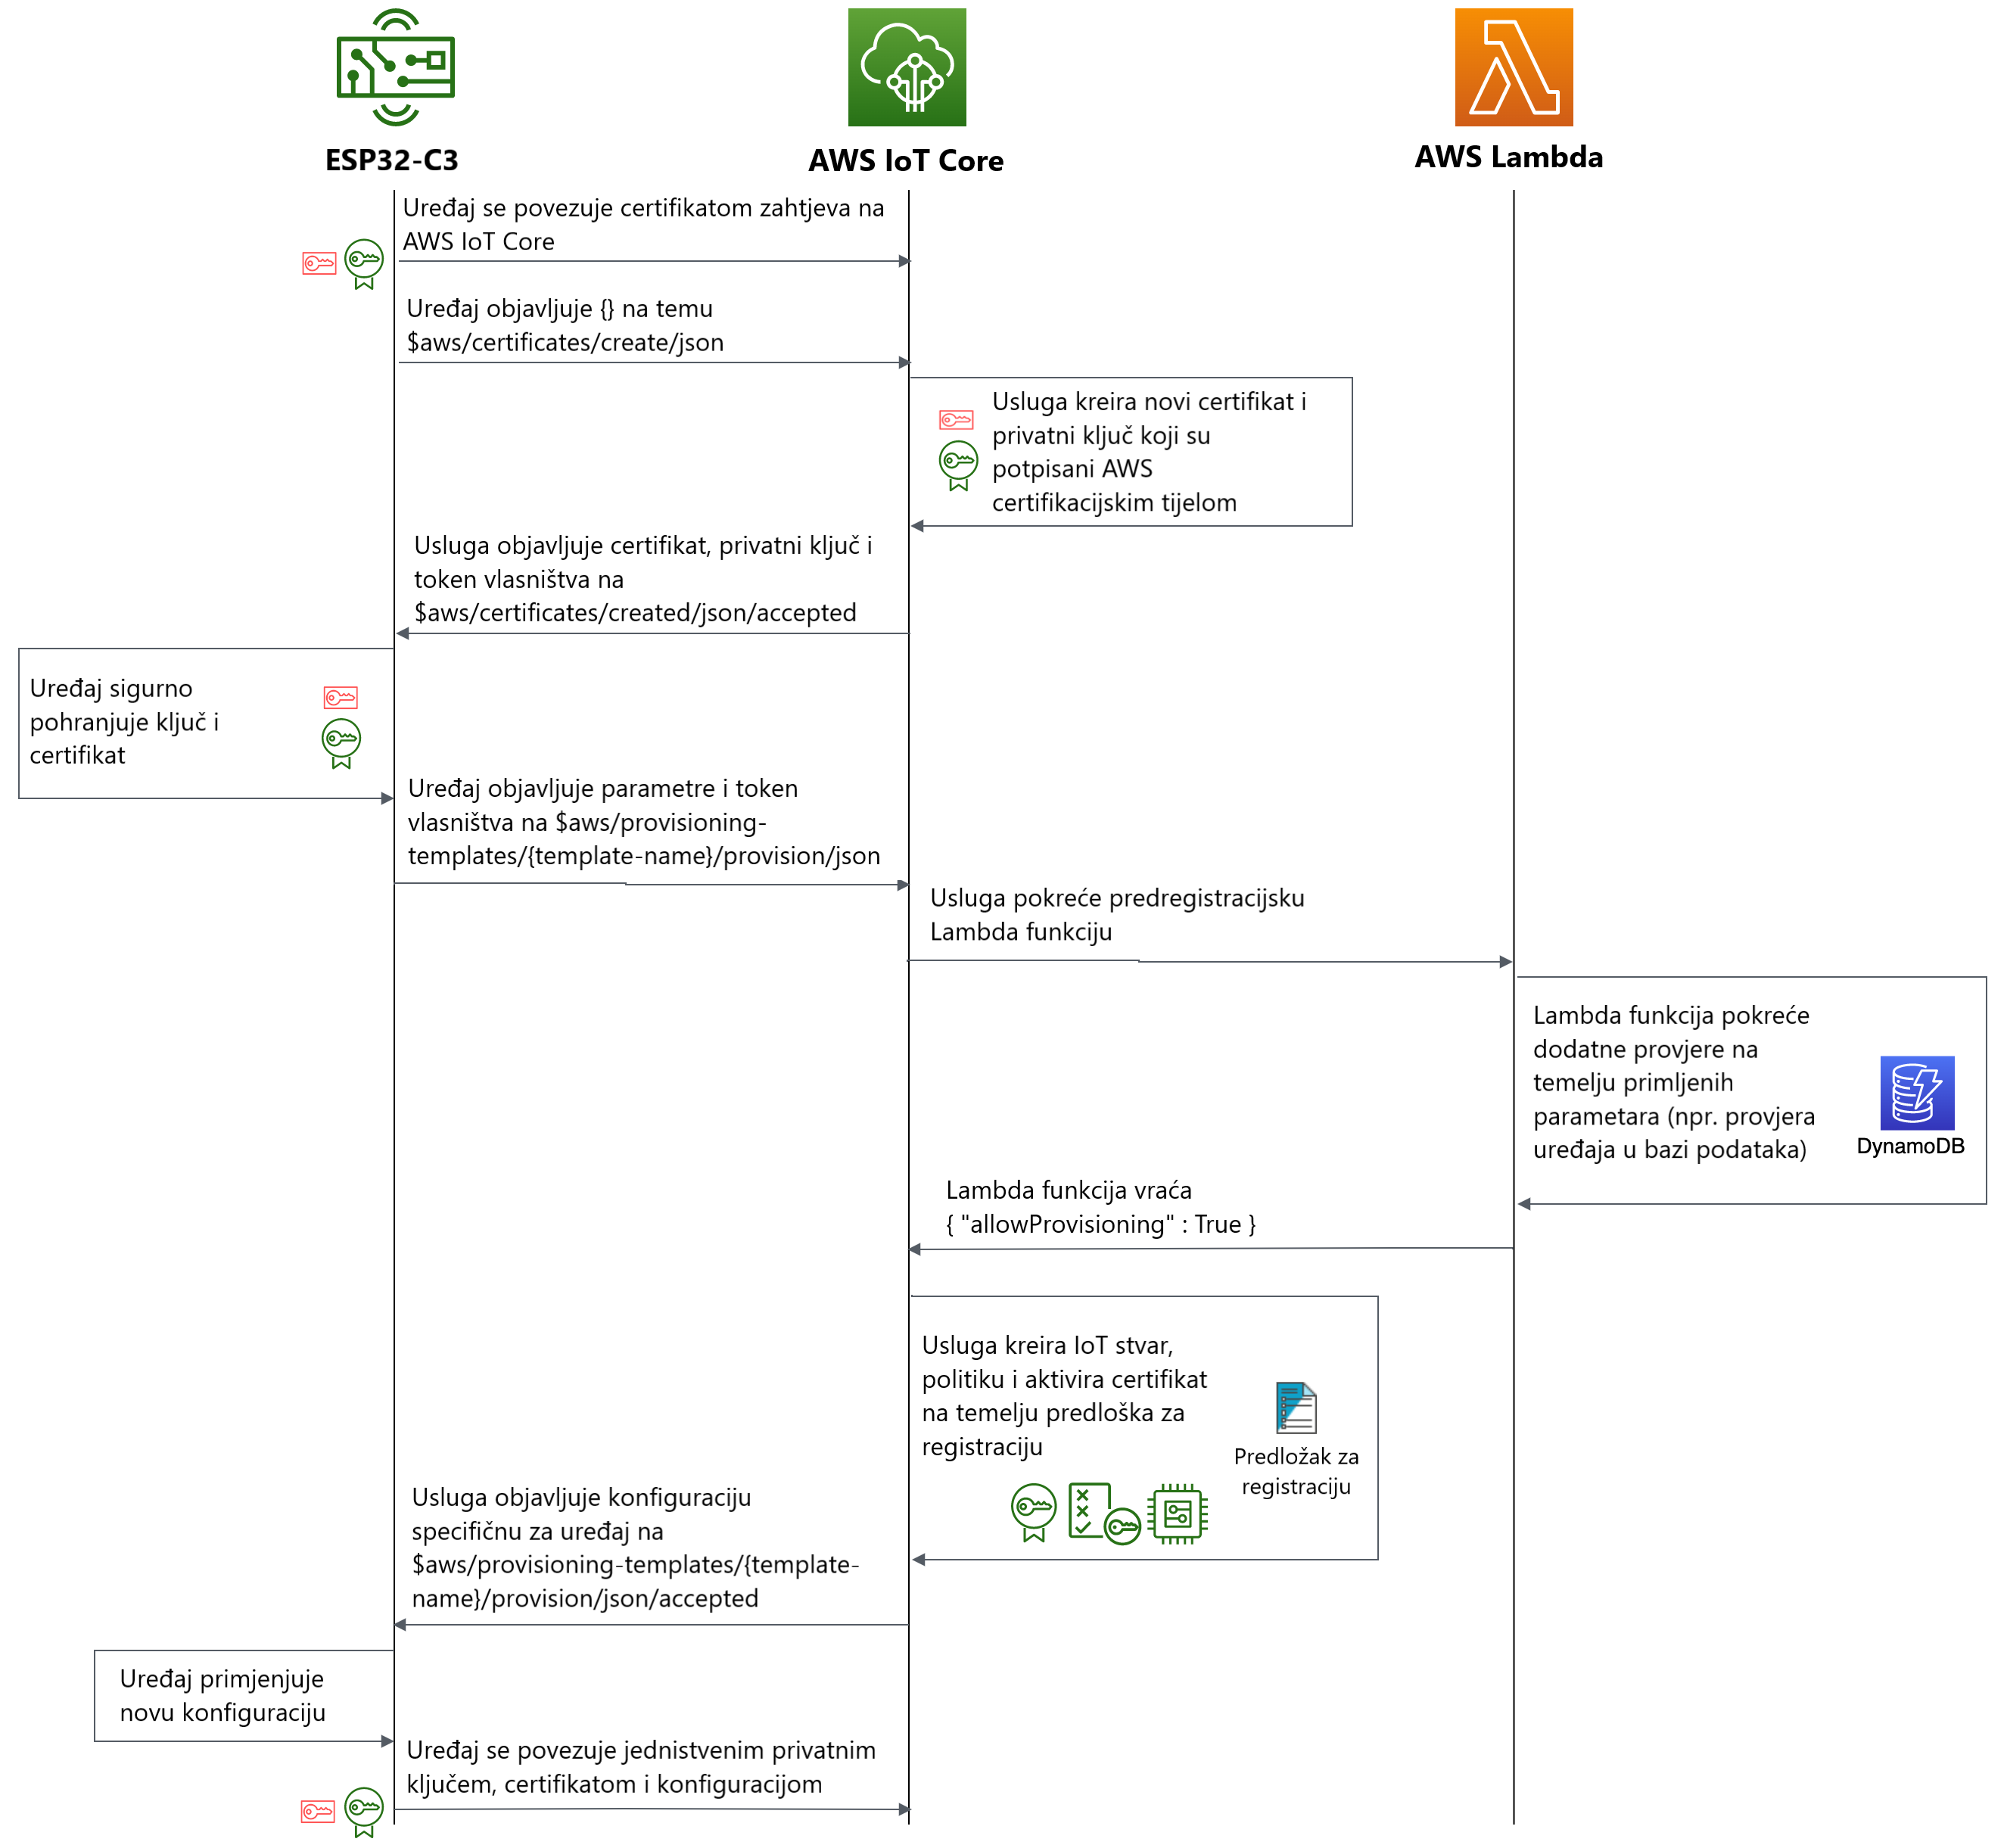
\includegraphics[scale=0.2]{imgs/fleet_provisioning_by_claim}
	\caption{Tok registracije uređaja certifikatom zahtjeva \cite{aws_docs}}
	\label{fig:fleet_provisioning_by_claim}
\end{figure}

Opisani tok ostvaren je uz pomoć ranije spomenute biblioteke, kao i knjižice \textit{coreMQTT} za komunikaciju putem protokola MQTT s API-jem platforme AWS. Za manipulaciju certifikatima i privatnim ključevima, korištena je biblioteka \textit{corePKCS11}. Ona koristi standard PKCS \#11 \engl{Public-key Certificate Standards}, što je široko korišten API za manipuliranje uobičajenim kriptografskim objektima. Funkcije koje navodi omogućuju aplikacijama korištenje, stvaranje, modificiranje i brisanje kriptografskih objekata, bez izlaganja tih objekata memoriji aplikacije. Primjerice, konkretna integracija s bibliotekom za registraciju uređaja koristi mali podskup PKCS \#11 API-ja za, između ostalog, pristup privatnom ključu potrebnom za stvaranje mrežne veze koja je autentificirana i zaštićena protokolom TLS bez da aplikacija ikada dođe u doticaj s ključem \cite{what_is_pkcs}. 

Sljedeći programski odsječak prikazuje uspostavu MQTT sjednice pomoću certifikata zahtjeva te podnošenje zahtjeva za novim certifikatom. U odsječku se također može primijetiti binarna serijalizacija podataka. Format CBOR \engl{Concise Binary Object Representation} Representation), za razliku od formata JSON, pretvara podatke u binarni oblik te ih tako šalje mrežom, što rezultira manjom latencijom i nosivošću \engl{payload} \cite{cbor}. Pri prijenosu velike količine podataka pri ograničenim resursima, poput u IoT sustava, ušteda na veličini poslanih podataka znatno utječe na efikasnost sustava. Isto tako, binaran je format prilagodljiv u odnosu na JSON, gdje mora postojati unaprijed definirana shema za primitak podataka.

\begin{lstlisting}[caption={Spajanje certifikatom zahtjeva i zahtjev za novim certifikatom}, language=c]
 LogInfo( ( "Establishing MQTT session with claim certificate..." ) );
 status = EstablishMqttSession( provisioningPublishCallback,
		*p11Session,
		pkcs11configLABEL_CLAIM_CERTIFICATE,
		pkcs11configLABEL_CLAIM_PRIVATE_KEY );
 status = subscribeToCsrResponseTopics();
 status = generateKeyAndCsr( *p11Session,
		pkcs11configLABEL_DEVICE_PRIVATE_KEY_FOR_TLS,
		pkcs11configLABEL_DEVICE_PUBLIC_KEY_FOR_TLS,
		csr,
		CSR_BUFFER_LENGTH,
		&csrLength );
/* Publish the CSR to CreateCertificatefromCsr API. */
 PublishToTopic( FP_CBOR_CREATE_CERT_PUBLISH_TOPIC,
		FP_CBOR_CREATE_CERT_PUBLISH_LENGTH,
		( char * ) payloadBuffer,
		payloadLength );
 status = waitForResponse();
\end{lstlisting}

\subsection{Očitavanje senzorskih mjerenja}

Razvijeni sustav, osim zaslona, sadrži dva senzora koja mjere stanja iz okoline: senzor za temperaturu i vlagu zraka te senzor za vlažnost tla. Mjerenja ovih senzora šalju se na platformu AWS i simuliraju stvarna poljoprivredna mjerenja. Mjerenje temperature i vlage zraka vrši se pomoću modula DHT11, dok se vlažnost tla mjeri senzorom VMA303. Tablice \ref{table:pinout_dht11} i \ref{table:pinout_vma} prikazuju konfiguracije spajanja senzora s razvojnim sustavom. 

\begin{table}[h]
	\centering
	\begin{minipage}{0.45\textwidth}
		\centering
		\begin{tabular}{|c|c|}
			\hline
			\rowcolor{lightblue}  
			\textbf{Pin ESP32-C3} & \textbf{Pin DHT11} \\ \hline
			GND & GND \\ \hline
			3.3V & Vcc \\ \hline
			GPIO 0 & S \\ \hline
		\end{tabular}
		\caption{Spajanje uređaja i modula DHT11}
		\label{table:pinout_dht11}
	\end{minipage}%
	\hspace{0.05\textwidth}
	\begin{minipage}{0.45\textwidth}
		\centering
		\begin{tabular}{|c|c|}
			\hline
			\rowcolor{lightblue}  
			\textbf{Pin ESP32-C3} & \textbf{Pin VMA303} \\ \hline
			GND & GND \\ \hline
			3.3V & Vcc \\ \hline
			GPIO 2 & S \\ \hline
		\end{tabular}
		\caption{Spajanje uređaja i senzora VMA303}
		\label{table:pinout_vma}
	\end{minipage}
\end{table}

Glavna funkcija senzora DHT11 jest mjerenje temperature i vlažnosti okoline. Senzor je tvornički kalibriran te može mjeriti temperaturu od 0°C do 50°C i vlažnost od 20\% do 90\% s točnošću od ±1°C i ±1\%. Senzor uključuje komponentu za mjerenje vlažnosti i NTC \engl{Negative Temperature Coefficient} komponentu za mjerenje temperature. DHT11 može se nabaviti kao senzor ili kao modul. Senzor dolazi kao 4-pinski paket od kojeg se koriste samo tri pina, dok modul dolazi s tri pina. Razlika između modula i senzora je u tome što modul ima ugrađeni kondenzator za filtriranje i otpornik za lakše spajanje s razvojnim sustavom \cite{dht11}. U razvijenom je sustavu korišten modul koji već ima integriran otpornik. 

Komunikacija i sinkronizacija između mikrokontrolera i senzora odvija se jednom podatkovnom linijom. Inicijalizacija komunikacije zahtijeva interakciju mikrokontrolera povlačenjem i otpuštanjem signala, čime jedan drugom signaliziraju spremnost na prijenos podataka. Najprije mikrokontroler povlači signal na nisku razinu na najmanje 18 milisekundi, nakon čega otpušta signal i pušta ga da se vrati na visoku razinu te čeka senzor da ga spusti natrag na nisku. DHT11 zatim povlači signal na nisku razinu na otprilike 80 mikrosekundi, nakon čega otpušta signal te se on vraća ponovno na visoku razinu, i taj proces također traje oko 80 mikrosekundi. Po završetku inicijalizacije DHT11 sekvencijalno prenosi 40 podatkovnih bitova, gdje prvi i treći bajt predstavljaju vlagu zraka i temperaturu. Drugi i četvrti bajt sadrže samo nule, a peti je kontrolni zbroj \engl{checksum} svih ostalih bajtova na sljedeći način:

\begin{lstlisting}[caption={Kontrolni zbroj poslanih bajtova s DHT11}, language=c]
	byte_5 == (byte_1 + byte_2 + byte_3 + byte_4) & 0xFF
\end{lstlisting}

Sensor VMA303 mjeri vlažnost tla tako što mjeri pad napona preko dvije elektrode. Senzor u sebi već ima integriran komparator, sto nije potrebno spajati dodatnu vanjsku komponentu. Osim elektroda, senzor se sastoji od kontrolnog elektronskog modula koji interpretira signale sa sonde i daje izlaz u digitalnom ili analognom obliku. Kada je sonda ubodena u tlo, metalne elektrode formiraju strujni krug. Vlažno tlo ima veću vodljivost što označava manji otpor, dok suho tlo ima manju vodljivost, time i veći otpor. Kontrolni modul šalje mali električni signal kroz jedan od pinova koji putuje kroz tlo i prima ga drugi pin. Na osnovu količine elektriciteta koji prođe kroz tlo, ovisno o vlažnosti zemlje, modul generira odgovarajući izlazni signal. U analognom načinu rada, modul daje izlazni napon proporcionalan nivou vlažnosti tla. Viša vlažnost rezultira višim naponom na izlaznom pinu, dok niža vlažnost daje niži napon. U slučaju digitalnog izlaza, modul koristi komparator za uspoređivanje izmjerene vrijednosti s unaprijed postavljenim pragom. Ako je vlažnost ispod praga, izlazni pin daje nisku razinu, dok u suprotnom vraća visoku razinu signala.

U razvijenom se sustavu koristi analogni način rada, te je potrebna analogno-digitalna pretvorba za analizu ulaznog signala. Pretvorba se odvija u jednokanalnom načinu rada te se koristi sukcesivna aproksimacija razlučivosti 12 bita. Sljedeći programski isječak prikazuje inicijalizaciju parametara ključnih za čitanje signala i pretvorbu. Vrijednosti \textit{DRY\_SOIL} i \textit{WET\_SOIL} označavaju najmanju i najveću moguću vrijednost pri mjerenju vlažnosti tla, odnosno 0\% i 100\%, te se stvarni postotak dobiva skaliranjem na te dvije vrijednosti i pretvaranjem u postotni oblik. Varijable su dobivene eksperimentalnim mjerenjem sirovih vrijednosti pri vlažnoj i suhoj zemlji. 

\begin{lstlisting}[caption={}, language=c]
void adc_init(void) {
	adc1_config_width(ADC_WIDTH);
}

void moisture_init() {
	adc1_config_channel_atten(MOISTURE_CHANNEL, ADC_ATTEN);
}

float read_moisture(void) {
	
	int adc_value = adc1_get_raw(MOISTURE_CHANNEL);
	float moisture = 0;
	
	if (adc_value >= WET_SOIL) {
		moisture = 100.0;
	} else if (adc_value <= DRY_SOIL) {
		moisture = 0.0;
	} else {
		moisture = ((100.0)/((double) DRY_SOIL - (double) WET_SOIL))*((double) (adc_value) - (double) WET_SOIL);
	}
	
	return moisture;
}
\end{lstlisting}

Senzorska mjerenja odvijaju se u posebnom FreeRTOS zadatku koji se pokreće nakon uspješnog povezivanja na Wi-Fi i registracije na platformu. Mjerenja se vrše svakih pet sekundi i prikazuju se na zaslonu. Isti se zadatak koristi i za slanje očitanih podataka nakon čitanja i prikaza. U nastavku je prikazan opisani zadatak. Također, može se primijetiti da isti zadatak pokreće funkciju za ažuriranje sjene uređaja. 

\begin{lstlisting}[caption={FreeRTOS zadatak za očitanje senzorskih mjerenja i slanje podataka}, language=c]
void publish_message_task(void *pvParameters) {
	float temperature, humidity, moisture;
	esp_err_t dht_temp;
	char display_text[512];
	
	while (1) {
		dht_temp = dht_read_float_data(SENSOR_TYPE, DHT_PIN, &humidity, &temperature) != ESP_OK;
		moisture = read_moisture();
		
		if (dht_temp == ESP_OK) {
			if (lvgl_port_lock(0)) {
			  lv_obj_t *screen = lv_scr_act();
			  lv_obj_clean(screen); // Clear the screen
			  lv_obj_t *label = lv_label_create(screen);
			  lv_label_set_long_mode(label,LV_LABEL_LONG_WRAP);
			  sprintf(display_text, "Temp: %.2f C\nHumid: %.2f%%\nMoist: %.2f%%", temperature, humidity, moisture);
			  lv_label_set_text(label, display_text);
			  // Release the mutex
			  lvgl_port_unlock();
			}
			sendMessage(temperature, humidity, moisture);
			color_name = device_shadow_main();
		}
		vTaskDelay(pdMS_TO_TICKS(5000));
	}
}
\end{lstlisting}

Slika \ref{fig:complete_device} prikazuje razvojni sustav ESP32-C3 spojen na periferne senzore te LCD zaslon. Isto tako, na zaslonu su vidljiva očitanja dobivena sa senzora. 

\begin{figure}[ht]
	\centering
	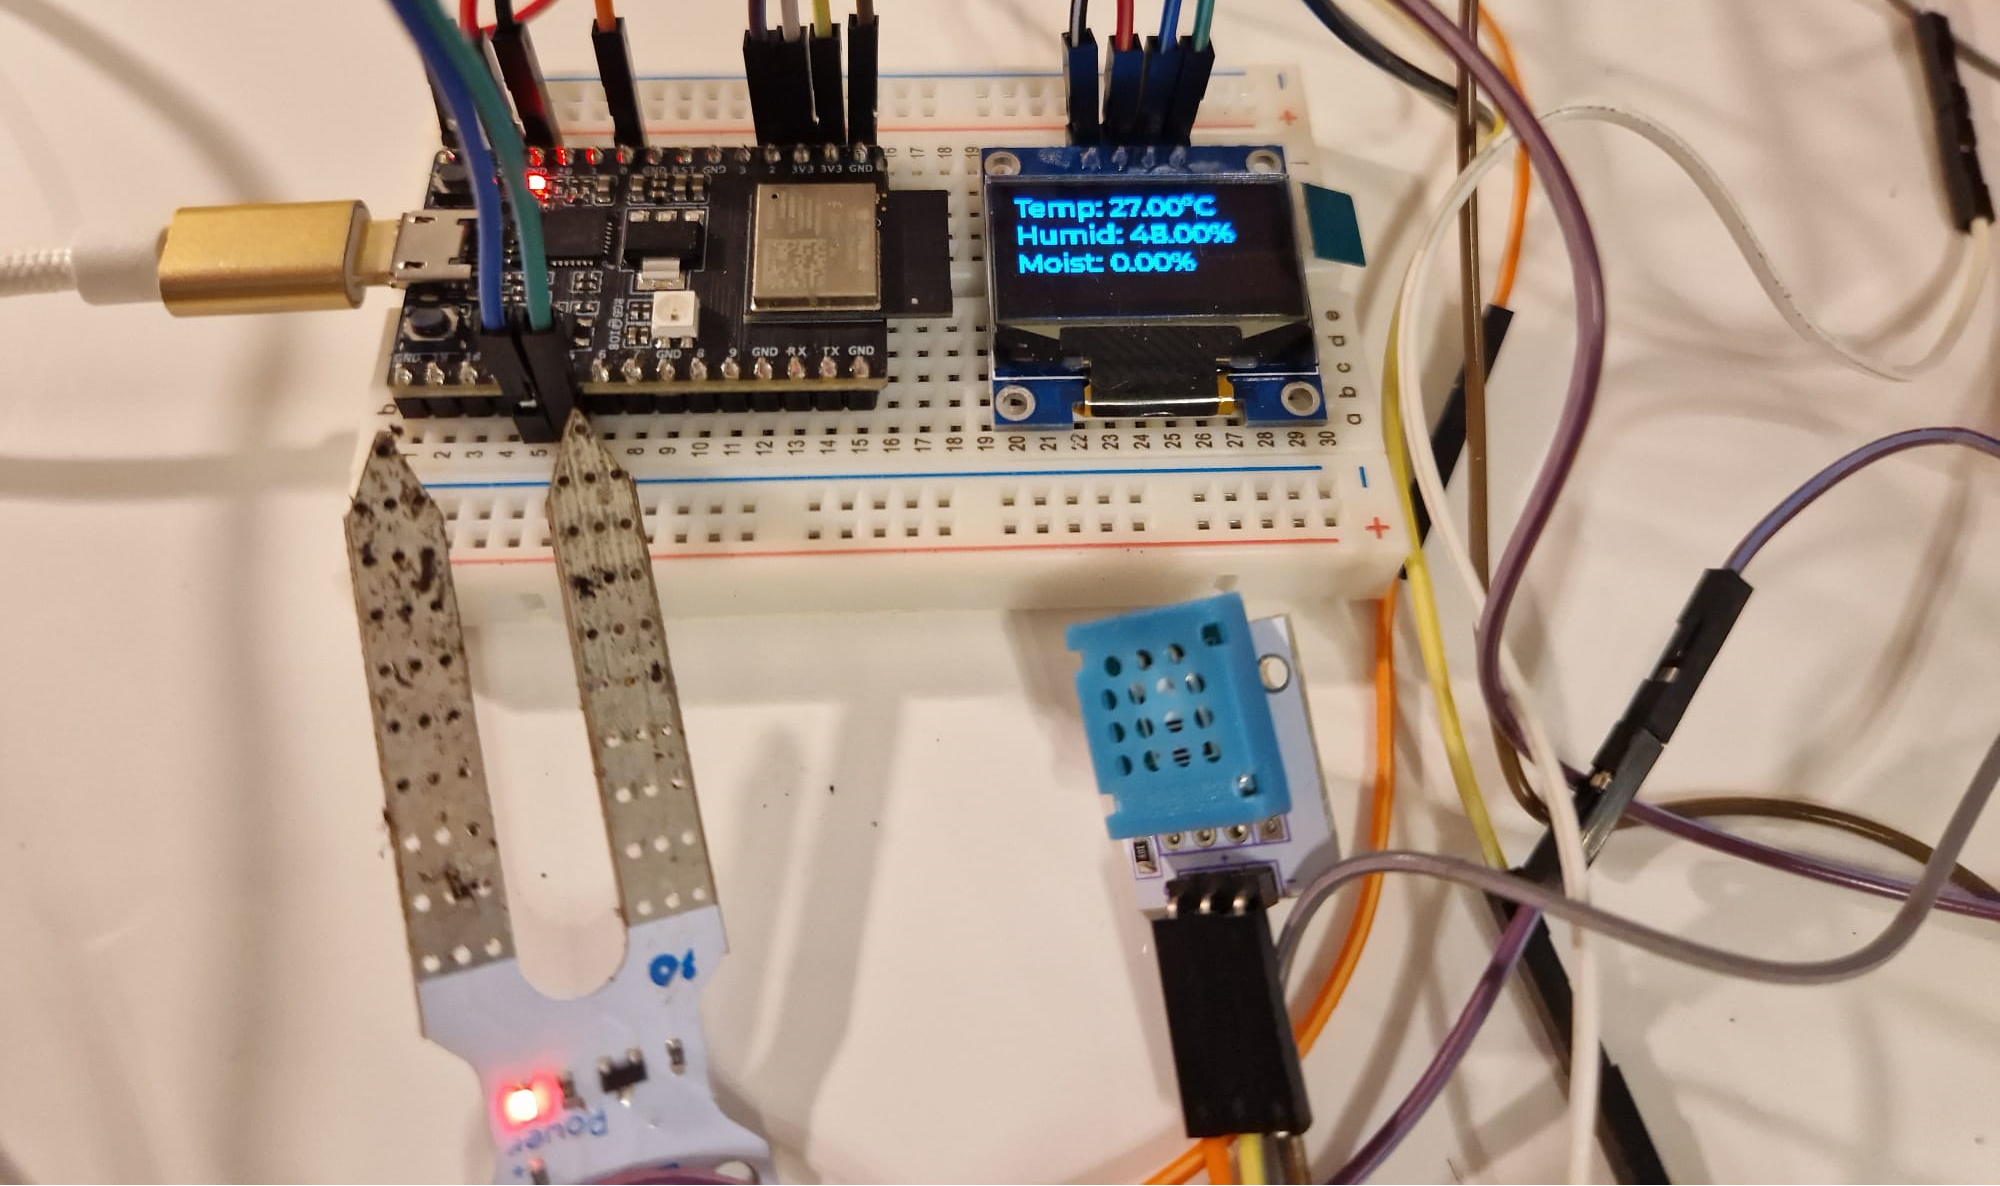
\includegraphics[scale=0.2]{imgs/complete_device}
	\caption{Razvojni sustav sa spojenom periferijom}
	\label{fig:complete_device}
\end{figure}

\subsection{Slanje očitanih podataka protokolom MQTT}

Kao što je ranije spomenuto, slanje očitanih podataka odvija se u istom zadatku odnosno dretvi kao i očitanje mjerenja, neposredno nakon dohvata vrijednosti. Slanje se odvija na temelju ranije ostvarene MQTT veze i razmijenjenim certifikatima. Podaci se šalju u formatu JSON radi jednostavnije kasnije obrade i čitljivosti pri primitku poruka. Za kreiranje podatkovne strukture za slanje korištena je biblioteka \textit{cJSON}. To je lagana i brza biblioteka za rukovanje podacima u obliku JSON namijenjena programskom jeziku C. Omogućava lako parsiranje, generiranje i manipulaciju JSON objekata te podržava sve tipove vrijednosti. Zbog jednostavne i optimizirane implementacije, nudi visoke performanse. Isto tako, ne oslanja se ni na kakve vanjske biblioteke, što je čini portabilnom u svim aplikacijama. Sljedeći programski isječak prikazuje funkcije za pripremanje objekta i njegovo slanje protokolom MQTT. Tema na koju šalje uređaj jest \lstinline[language=c]|device/{clientIdentifier}/data|, gdje je identifikator zapravo serijski naziv uređaja. Time je osigurano da svaki uređaj šalje na točno odgovarajuću temu. Koristi se kvaliteta usluge 0 \engl{Quality of Service - QoS} bez potvrde prijema jer se podaci šalju svakih pet sekundi, a senzorska mjerenja se ne mijenjaju drastično u tako kratkom periodu, stoga si razvijeni sustav može priuštiti povremeni gubitak poruka. Ovim se načinom također štedi vrijeme čekanja i resursi koji su korištenom razvojnom sustavu potrebni.  

\begin{lstlisting}[caption={Funkcije za pripremanje JSON objekta i njegovo slanje protokolom MQTT}, language=c]
void prepareJSONMessage(float temperature, float humidity, float moisture, uint8_t *buffer, size_t *length) {
	// Create the main JSON object
	cJSON *jsonObject = cJSON_CreateObject();
	
	struct timeval now;
	gettimeofday(&now, NULL);
	int64_t time_in_ms = (int64_t)now.tv_sec * 1000 + now.tv_usec / 1000;
	cJSON_AddNumberToObject(jsonObject, "timestamp", time_in_ms);
	
	cJSON_AddStringToObject(jsonObject, "device_id", CLIENT_IDENTIFIER);
	
	// Create a nested JSON object for data
	cJSON *dataObject = cJSON_CreateObject();
	cJSON_AddNumberToObject(dataObject, "temperature", temperature);
	cJSON_AddNumberToObject(dataObject, "humidity", humidity);
	cJSON_AddNumberToObject(dataObject, "moisture", moisture);
	
	// Add the data object to the main JSON object
	cJSON_AddItemToObject(jsonObject, "data", dataObject);
	
	// Print the JSON object to a string
	char *jsonString = cJSON_PrintUnformatted(jsonObject);
	
	// Copy the JSON string to the buffer and set the length
	*length = strlen(jsonString);
	memcpy(buffer, jsonString, *length);
	
	// Clean up
	cJSON_Delete(jsonObject);
	cJSON_free(jsonString); // free the allocated string
}

void sendMessage(float temperature, float humidity, float moisture) {
	prepareJSONMessage(temperature, humidity, moisture, payloadBuffer, &payloadLength);
	bool status = false;
	
	status = PublishToTopic( MQTT_DATA_TOPIC,
	MQTT_DATA_TOPIC_LENGTH,
	( char * ) payloadBuffer,
	payloadLength );
	
	if( status == false )
	{
		LogError( ( "Failed to publish to topic: %.*s.",
		MQTT_DATA_TOPIC_LENGTH,
		MQTT_DATA_TOPIC ) );
	}
	
}
\end{lstlisting}

Iz prve funkcije vidljivo je da uređaj u JSON objekt pohranjuje očitane vrijednosti temperature, vlage zraka te vlažnosti tla. Također, šalje identifikator uređaja kako bi se naznačilo koji uređaj šalje podatke. Isto tako, šalje se i vremenska oznaka, što je pogodno za buduću obradu i analizu podataka. Budući da mikrokontroler interno mjeri vrijeme od početka prvog pokretanja nakon instalacije \textit{firmwarea}, potrebno je sinkronizirati njegov interni sat s lokalnim vremenom. Kako bi se osigurano točno vrijeme, mikrokontroler se povezuje na SNTP poslužitelj. Protokol SNTP \engl{Simple Network Time Protocol} jest protokol koji omogućava uređajima da se sinkroniziraju s mrežnim vremenskim poslužiteljima kako bi dobili precizno vrijeme \cite{sntp}. Budući da je uređaj ranijim procesima već spojen na Wi-Fi, potrebno je korištenjem gotove biblioteke tvrtke \textit{Espressif} spojiti se na poslužitelj te dohvatiti trenutno vrijeme i sinkronizirati vlastito u skladu s dohvaćenim. Uređaj se spaja na \lstinline|pool.sntp.org| što je domensko ime za globalni mrežni projekt koji pruža vremenske poslužitelje za sinkronizaciju vremena putem protokola NTP \engl{Network Time Protocol}. Ovu je sinkronizaciju potrebno napraviti samo jednom, i to nakon spajanja na internet. Sljedeći programski isječak prikazuje funkciju koja se spaja na poslužitelj i obavlja sinkronizaciju. Ugrađen je i mehanizam pokušaja ponovnog spajanja svake dvije sekunde u najviše deset iteracija ukoliko prvotno spajanje i dohvat nisu uspješni.

\begin{lstlisting}[caption={Funkcije za sinkronizaciju vremena s SNTP poslužiteljem}, language=c]
void initialize_sntp(void)
{
	ESP_LOGI(TAG, "Initializing SNTP");
	esp_sntp_setoperatingmode(SNTP_OPMODE_POLL);
	esp_sntp_setservername(0, "pool.ntp.org");
	sntp_set_time_sync_notification_cb(time_sync_notification_cb);
	esp_sntp_init();
}

void obtain_time(void)
{
	initialize_sntp();
	
	// Wait for time to be set
	time_t now = 0;
	struct tm timeinfo = { 0 };
	int retry = 0;
	const int retry_count = 10;
	
	while (timeinfo.tm_year < (2024 - 1900) && ++retry < retry_count) {
		ESP_LOGI(TAG, "Waiting for system time to be set... (%d/%d)", retry, retry_count);
		vTaskDelay(2000 / portTICK_PERIOD_MS);
		time(&now);
		localtime_r(&now, &timeinfo);
	}
	
	if (retry < retry_count) {
		ESP_LOGI(TAG, "Time synchronized successfully");
	} else {
		ESP_LOGE(TAG, "Failed to synchronize time");
	}
}
\end{lstlisting}

Nakon generiranja JSON objekta, ovako izgleda konačan objekt koji uređaj šalje AWS-u:

\begin{lstlisting}[caption={JSON objekt za slanje na platformu}, language=json]
{
	"timestamp": 123456789,
	"device_id": "serialNumber123",
	"data": {
		"temperature": 23.00,
		"humidity": 55.00,
		"moisture": 62.00
	}
}
\end{lstlisting}

\subsection{Sjena uređaja}

Budući da nije kreirana nikakva dodatna aplikacija koja bi koristila sjenu uređaja i tražila zahtjev za promjenom stanja odnosno sjene, uređaj sam sebi šalje zahtjev za promjenom i isto tako šalje i ažurirano stanje. Promjenjivo stanje uređaja simulirano je bojom LED diode koja konstantno treperi periodom od dvije sekunde.  

LED dioda integrirana je u razvojni sustav i vrsta je adresirajuće LED diode. Takve diode mogu se pojedinačno kontrolirati unutar trake ili matrice, čime su omogućeni složeni svjetlosni efekti i uzorci. Za razliku od običnih LED dioda koje se mogu samo uključiti ili isključiti, adresirajuće LED diode imaju integrirane upravljačke čipove koji omogućuju svakom pikselu u traci da primi jedinstvenu naredbu \cite{led}. Pri upravljanju LED diodom, koristi se način rada RMT \engl{Remote Control Transceiver}. To je periferni sklop koji služi kao infracrveni primopredajnik. Međutim, zbog fleksibilnosti formata podataka, RMT se može proširiti na svestrani primopredajnik opće namjene, koji odašilje ili prima i druge vrste signala. Iz perspektive slojevitosti mreže, hardver sadrži i fizički i sloj podatkovne veze. Fizički sloj definira komunikacijski medij i reprezentaciju signala bita, dok sloj podatkovne veze definira format RMT okvira. Ovaj periferni sklop koristi se za generiranje i dekodiranje nizova impulsa, što ga čini prikladnim za zadatke koji uključuju precizno mjerenje vremena, kao što je pokretanje adresirajućih LED dioda. One zahtijevaju striktno vremensko određivanje kako bi ispravno protumačile podatkovne signale \cite{espressif}. 

RMT hardver ima vlastiti format uzorak podataka zvan RMT simbol. Svaki simbol sastoji se od dva para po dvije vrijednosti. Prva vrijednost u paru je 15-bitna vrijednost koja predstavlja trajanje signala u jedinicama RMT taktova. Druga u paru je 1-bitna vrijednost koja predstavlja logičku razinu signala, tj. visoku ili nisku. Slika \ref{fig:rmt} prikazuje način na koji funkcionira RMT odašiljač. Upravljački program kodira korisničke podatke u format podataka tipa RMT, i zatim odašiljač može generirati valne oblike prema artefaktima kodiranja. Također je moguće modulirati visokofrekventni nosivi signal prije usmjeravanja na GPIO izlaze.

\begin{figure}[ht]
	\centering
	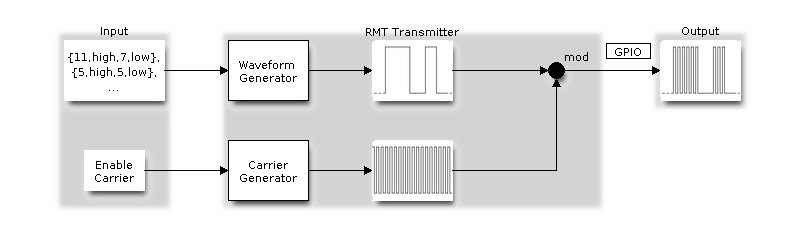
\includegraphics[scale=0.5]{imgs/rmt}
	\caption{Pregled RMT odašiljača \cite{espressif}}
	\label{fig:rmt}
\end{figure}

Sljedeći programski isječak prikazuje konfiguraciju LED diode kao i zadatak koji vrši treperenje. Koristi se biblioteka \textit{led\_strip}, što je službeni upravljački program \engl{driver} za adresirajuće LED diode u modulima ESP32. Konfiguraciji se pridjeljuje GPIO pin na kojem se nalazi dioda te se postavlja razlučivost RMT signala na 10 MHz. Ovo određuje vremensku preciznost signala poslanih LED diodi. Isto tako, moguće je koristiti izravan pristup memoriji \engl{Direct Memory Access - DMA}, no u ovom slučaju nije potreban. U glavnom je programu kreiran poseban FreeRTOS zadatak za treperenje LED diode. Kreirana je posebna struktura \lstinline|color_t| koja predstavlja boju u RGB formatu i odabrana se boja prosljeđuje funkciji \lstinline|blink_led()|. Također, kreirana je posebna funkcija koja na temelju tekstualne riječi boje generira boju u RGB formatu. U razvijenom sustavu podržane su sljedeće boje: crvena, zelena, plava, žuta, ljubičasta i bijela. Parametar \lstinline|color_name| globalna je varijabla koja se postavlja u zadatku koji izvršava slanje poruka i ažuriranje sjene uređaja. 

\begin{lstlisting}[caption={Upravljanje LED diodom}, language=c]
typedef struct {
		uint8_t r;
		uint8_t g;
		uint8_t b;
} color_t;

static void configure_led()
{
	led_strip_config_t strip_config = {
		.strip_gpio_num = BLINK_GPIO,
		.max_leds = 1, // at least one LED on board
	};
	led_strip_rmt_config_t rmt_config = {
		.resolution_hz = 10 * 1000 * 1000, // 10MHz
		.flags.with_dma = false,
	};
	ESP_ERROR_CHECK(led_strip_new_rmt_device(&strip_config, &rmt_config, &led_strip));
	led_strip_clear(led_strip);
}

static void blink_led(uint8_t s_led_state, color_t color)
{
	if (s_led_state) {
		led_strip_set_pixel(led_strip, 0, color.r, color.g, color.b);
		led_strip_refresh(led_strip);
	} else {
		led_strip_clear(led_strip);
	}
}

void blinky_task(void *pvParameters) {
	uint8_t s_led_state = 0;
	color_t color;
	
	configure_led();
	
	while (1) {
		if (s_led_state == true) {
			color = get_color_from_string(color_name);
		}
		
		blink_led(s_led_state, color);
		s_led_state = !s_led_state;
		vTaskDelay(1000 / portTICK_PERIOD_MS);
	}
}
\end{lstlisting}

Kao što je ranije spomenuto, uređaj najprije generira zahtjev za promjenom stanja, odnosno pošalje željeno stanje AWS-u i na temelju tog zahtjeva mijenja stvarno stanje i prijavljuje ga. Željeno je stanje nasumičan odabir jedne od ranije navedenih boja u tekstualnom obliku. Razvijeni sustav koristi samo jednu sjenu uređaja, i to klasičnu. Svaka tema vezana za sjenu uređaja povezana je sa stvari odnosno njezinim imenom, te se slanjem na pojedinačne teme podrazumijeva da je u temu integriran naziv stvari o čijoj se sjeni uređaja radi. Funkcionalnost sjene uređaja funkcionira na sljedeći način: najprije, uređaj pokušava obrisati sjenu ako postoji. Za to se mora pretplatiti na teme \textit{/delete/accepted} i \textit{/delete/rejected} te objaviti na temu \textit{delete} i primati poruke na pretplaćenim temama. Brisanje se smatra uspješnim u ova dva slučaja:
\begin{itemize}
	\item poruka je stigla na temu \textit{/delete/accepted},
	\item poruka je stigla na temu \textit{/delete/rejected} s greškom 404, što znači da pri pokušaju brisanja sjena uređaja ne postoji.
\end{itemize}

Uređaj se nakon uspješnog brisanja odjavljuje s pretplaćenih tema i prijavljuje se na teme za ažuriranja sjene uređaja. Zatim uređaj nasumično generira boju koja će predstavljati željeno stanje uređaja i šalje je na temu \textit{/update}, na koju je ujedno i pretplaćen. Ta ista poruka stigne na pretplaćenu temu i uređaj ažurira trenutnu boju LED diode u diodu željenog stanja i zatim šalje prijavljeno stanje na platformu. Verzije sjene uređaja automatski se povećavaju za jedan. Isto tako, svaki zahtjev ima vlastiti klijentski token koji je postavljen na serijski broj uređaja. Time je osigurano da se sjene različitih uređaja ne miješaju, nego da uređaj samom sebi šalje zahtjev. Po primitku željene poruke, program provjerava odgovara li klijentski token vlastitom tokenu, te u tom slučaju odobrava promjenu stanja, mijenja boju LED diode i šalje platformi novo prijavljeno stanje. Sljedeći programski isječak prikazuje skraćenu verziju opisanog procesa pretplate, brisanja sjene, odjave, ponovne pretplate te objave ažuriranja sjene uređaja. Iz isječka se može vidjeti da se, za razliku od slanja podataka, proces komunikacije s platformom vezano za sjenu uređaja odvija kvalitetom usluge QoS1, što znači da sustav čeka odgovor na poruku. Time se osigurava da će se stanje stvarno ažurirati na novu vrijednost.  

\begin{lstlisting}[caption={Proces ažuriranja sjene uređaja}, language=c]
LogInfo( ( "Sub to `/delete/accepted` and `/delete/rejected` topics." ) );
status = SubscribeToTopic( SHADOW_TOPIC_STR_DELETE_ACC( THING_NAME, SHADOW_NAME ),
	SHADOW_TOPIC_LEN_DELETE_ACC( THING_NAME_LENGTH, SHADOW_NAME_LENGTH ) );
status = SubscribeToTopic( SHADOW_TOPIC_STR_DELETE_REJ( THING_NAME, SHADOW_NAME ),
	SHADOW_TOPIC_LEN_DELETE_REJ( THING_NAME_LENGTH, SHADOW_NAME_LENGTH ) );
LogInfo( ( "Publish to `delete` topic to try to delete the shadow doc." ) );
status = PublishToTopicQoS1( SHADOW_TOPIC_STR_DELETE( THING_NAME, SHADOW_NAME ), 
	SHADOW_TOPIC_LEN_DELETE( THING_NAME_LENGTH, SHADOW_NAME_LENGTH ),
	updateDocument,
	0U );
			
/* Unsubscribe from topics... */
/* Subscribe to /update/delta topics... */

LogInfo( ( "Send desired color." ) );
( void ) memset( updateDocument,
	0x00,
	sizeof( updateDocument ) );

const char* randomColor = get_random_color_string();

snprintf( updateDocument,
	SHADOW_DESIRED_JSON_LENGTH + 1,
	SHADOW_DESIRED_JSON,
	randomColor,
	clientToken );

status = PublishToTopicQoS1( SHADOW_TOPIC_STR_UPDATE( THING_NAME, SHADOW_NAME ),
	SHADOW_TOPIC_LEN_UPDATE( THING_NAME_LENGTH, SHADOW_NAME_LENGTH ),
	updateDocument,
	( SHADOW_DESIRED_JSON_LENGTH + 1 ) );
\end{lstlisting}

Slika \ref{fig:rgb_lights} prikazuje nekoliko različitih boja LED diode koje se kontroliraju sjenom uređaja. 

\begin{figure}[ht]
	\centering
	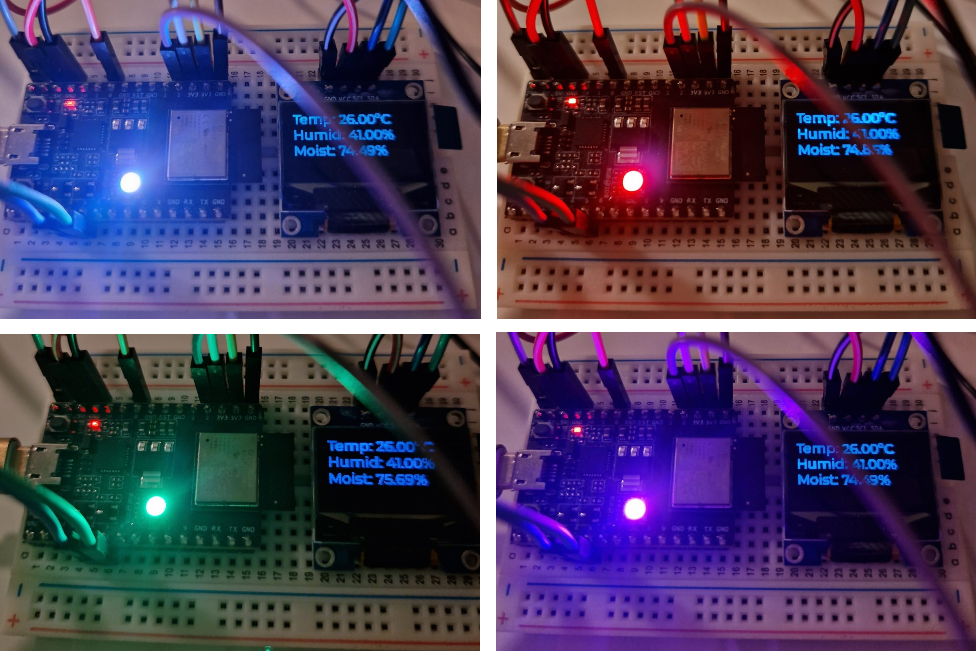
\includegraphics[scale=0.5]{imgs/rgb_lights}
	\caption{Različite boje LED diode}
	\label{fig:rgb_lights}
\end{figure}

\subsection{Ažuriranje softvera}

Programska potpora za ažuriranje softvera koristi OTA biblioteku u sklopu ranije spomenutog razvojnog paketa za integraciju platforme AWS i ESP32 uređaja. Primaju se MQTT poruke koje se prosljeđuju OTA agentu za moguću obradu. OTA agent koji je već razvijen u sklopu biblioteke obavlja glavni dio posla i provjerava je li mu dolazna MQTT poruka zapravo namijenjena. 

\section{Programska potpora za oblak}

Programska potpora za platformu AWS većim dijelom nije kod u standardnom smislu, no kako bi se uređaj i platforma uopće mogli komunicirati međusobno, potrebno je omogućiti povezivanje i komunikaciju na samoj platformi. Sva se komunikacija odvija u istoj AWS regiji. Zbog dostupnosti većine IoT usluga i relativne geografske bliskosti, korištena je regija \textit{eu-north-1} odnosno Stockholm, Švedska. 

Isto tako, važno je istaknuti kako se sve opisane radnje u sustavu AWS mogu izvršavati pomoću naredbenog retka platforme AWS \engl{Command-line interface - CLI}, no radi jednostavnosti i preglednosti, korišteno je korisničko sučelje platforme.

Programska potpora sastoji se od sljedećih segmenata:
\begin{itemize}
	\item omogućavanje dinamičke registracije uređaja,
	\item slanje novog softvera na uređaj,
	\item pristup zadnjem stanju uređaja nakon gubitka veze,
	\item obrada podataka dobivenih protokolom MQTT,
	\item pohrana podataka.
\end{itemize}

\subsection{Dinamička registracija uređaja}

Kao što je ranije opisano, u razvijenom sustavu koriste se certifikati zahtjeva za prvotno spajanje na platformu AWS, stoga je potrebno kreirati odgovarajući predložak za registraciju. Predložak također mora imati dodijeljenu politiku koja autorizira certifikat zahtjeva i ta se politika dodjeljuje generiranim certifikatima zahtjeva. Odabiru se politike koje omogućavaju točno onoliko koliko je potrebno za spajanje u sustav, a to su dopuštenja za MQTT komunikaciju i spajanje na AWS. Također, potrebno je odabrati koji su certifikati valjani kao zahtjev. Poželjno je i dodijeliti Lambda funkciju kao predregistracijsku provjeru dodatne valjanosti zahtjeva i poslanih parametara. Za razvijeni sustav nije kreirana Lambda funkcija, što znači da je svaki zahtjev automatski odobren. Isto tako, moguće je automatski pri registraciji uređaja kreirati i pripadnu stvar \engl{thing}, što je korisno za kasniju organizaciju i pregled certifikata. Svaka stvar može imati modularan naziv, ovisno o parametrima koji se pošalju. Za ovaj sustav postavljen je prefiks \textit{ESP32Thing\_} koji označava da su uređaji vrste ESP32, a ostatak naziva stvari ovisi o serijskom broju samog uređaja. To osigurava da svaki uređaj kreira jedinstvenu stvar u AWS-u. Moguće je odabrati i vrstu stvari \engl{thing type} koja će se automatski pridijeliti stvari, te u ovom slučaju kreirana je nova vrsta stvari naziva ESP32-C3. Stvarima se može dodijeliti i grupa, no u ovom sustavu nije bilo potrebe za kreiranjem dodatne grupe stvari budući da se povezuje samo jedna vrsta uređaja u sustav. Naposlijetku, potrebno je odabrati koje će se politike dodijeliti novogeneriranom jedinstvenom certifikatu, čime će uređaj dobiti pristup uslugama sustava AWS. Odabrane politike u ovom sustavu imaju sva dopuštenja radi lakše demonstracije funkcionalnosti. U nastavku se može vidjeti isječak kreiranog predloška, odnosno parametri stvari koja se kreira korištenjem predloška. U odsječku se isto tako može vidjeti funkcija za kreiranje imena stvari koja koristi predefinirani prefiks i serijski broj uređaja. 

\begin{lstlisting}[caption={Odjeljak \textit{stvar} u predlošku za registraciju}, language=json]
 "thing": {
	"Type": "AWS::IoT::Thing",
	"OverrideSettings": {
		"AttributePayload": "MERGE",
		"ThingGroups": "DO_NOTHING",
		"ThingTypeName": "REPLACE"
	},
	"Properties": {
		"AttributePayload": {},
		"ThingGroups": [],
		"ThingName": {
			"Fn::Join": [
			"",
			[ "ESP32Thing_", { "Ref": "SerialNumber" } ]
			]
		},
		"ThingTypeName": "ESP32-C3"
	}
 }
\end{lstlisting}

Na slici \ref{fig:policies} nalazi se popis politika koje su dodijeljene uređaju registriranom u sustav. Omogućene su sve politike, odnosno dodijeljene su sve dozvole koje uređaj može imati. Politika \textit{DevicePolicy} odnosi se na komunikaciju MQTT protokolom, \textit{DeviceShadowPolicy} na akcije vezane uz sjenu uređaja, \textit{JobPolicy} na izvršavanje i dohvat poslova te \textit{CertificatePolicy} dozvoljava povezivanje certifikatom. 

\begin{figure}[ht]
	\centering
	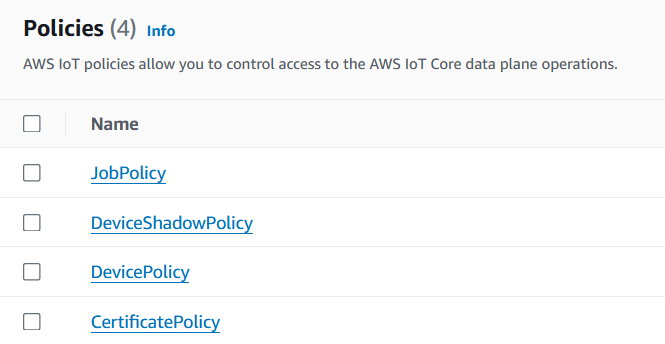
\includegraphics[scale=0.8]{imgs/policies}
	\caption{Popis politika dodijeljenih registriranom uređaju}
	\label{fig:policies}
\end{figure}

\subsection{Obrada i pohrana dobivenih podataka}

Podaci poslani protokolom MQTT u ranije prikazanom formatu JSON šalju se platformi na određenu temu definiranu serijskim nazivom uređaja. Svi se podaci šalju sigurno uspostavljenom vezom na vrata 8883 i krajnju točku brokera koju AWS generira ovisno o regiji kojoj se šalju podaci. Korištenjem testnog klijenta koji nudi AWS i pretplatom na željene teme moguće je u stvarnom vremenu pratiti podatke koji uređaj šalje. 

Primljeni se podaci moraju pohraniti u bazu podataka kako bi se kasnije mogli koristiti za pregled i analizu. AWS nudi uslugu preusmjeravanja poruka \engl{message routing} protokom podataka između povezanih uređaja i aplikacija. Koristi pravila za usmjeravanje \engl{rules engine} kako bi obradila i preusmjerila poruke koje dolaze s uređaja prema drugim uslugama ili vanjskim krajnjim točkama. Moguće je usmjeriti poruke izravno prema sustavima za pohranu koji se nude u sklopu AWS usluga, no isto tako i prema Lambda funkcijama koje mogu vršiti detaljniju obradu podataka. Pravila usmjeravanja definiraju se SQL upitima nad MQTT temama, čime se omogućava filtriranje, transformacija i usmjeravanje podataka na osnovu specifičnih kriterija. Upitima je moguće izdvojiti specifična polja iz JSON poruka ili pak računati nove vrijednosti na temelju dobivenih. 

Svaka ruta mora imati jedinstveno ime te upit kojim se dohvaćaju podaci. Upit je standardan SQL upit, no izvor podataka je tema na koju dolaze poruke u AWS. Unutar tema također je moguće koristiti i zamjenske znakove \engl{wildcards} kako bi upit odgovarao više tema. U razvijenom sustavu korišten je upit koji obuhvaća sve teme na koje uređaji šalju svoje podatke, neovisno o serijskom broju uređaja.

\begin{lstlisting}[caption={SQL upit rute za podatke s uređaja}, language=sql]
	SELECT * FROM 'device/+/data' 
\end{lstlisting}

Nadalje, potrebno je odabrati kamo će se odabrani podaci slati. Dobivene je podatke moguće slati u zapise \engl{logs}, metrike, u baze podataka unutar AWS-a, na novu MQTT temu, ili pak preusmjeriti podatke Lambda funkciji. Iako AWS nudi direktno slanje u baze podataka, poput baze DynamoDB, ovo rješenje nije odabrano zbog kompliciranog dohvata podataka i njihove vizualizacije u korištenoj web aplikaciji. Stoga se podaci preusmjeravaju na Lambda funkciju koja vrši daljnju obradu i slanje podataka u bazu. 

Još jedna od usluga platforme AWS jest Amazon Timestream koja nudi potpuno upravljane baze podataka vremenskih serija za radna opterećenja od upita niske latencije pa sve do unosa velikih podataka. Usluga je namijenjena podacima koji sadrže vremensku oznaku za analizu vremenskih serija. Automatski skalira kapacitet prema potrebi, čime omogućava rukovanje mnoštvom podataka bez ručnog dodavanja resursa. Arhitektura je dizajnirana tako da omogućava brzi unos i pokretanje upita, pružajući visoku propusnost i nisku latenciju. Također, automatizira procese arhiviranja i upravljanja podacima. Korisnici mogu definirati politike zadržavanja podataka kako bi se stari podaci automatski premjestili u jeftinijem i sporijem spremniku za pohranu, dok noviji podaci ostaju u pohrani brzog pristupa. Time se optimiziraju troškovi i performanse bez ručne intervencije. U sklopu usluge Amazon Timestream nude se dvije baze podataka vremenskih serija: LiveAnalytics i InfluxDB. Baza LiveAnalytics primarno je namijenjena podacima koji zahtijevaju detaljnu analizu i praćenje velike količine podataka u stvarnom vremenu. Ima ugrađene analitičke funkcije za praćenje trendova i uzoraka. Isto tako, pogodna je za pohranu zapisa i događaja. InfluxDB je baza podataka otvorenog koda, što je čini fleksibilnijom pri konfiguraciji u odnosu na LiveAnalytics. Baza je pogodna za pohranu metrika i očitanja s IoT uređaja \cite{aws_docs}. Kao što je opisano, obje baze podataka pripadaju skupini baza vremenskih serija, koje spadaju u skupinu NoSQL bazi podataka. Takve baze pohranjuju podatke u strukturi drukčijoj od klasičnih relacijskih modela, primjerice u formatu JSON s parovima ključ-vrijednost. NoSQL sustavi nastali su iz novih zahtjeva za većom fleksibilnošću i boljim performansama u pohrani i obradi velike količine podataka, uglavnom zbog popularnosti interneta i internetskih tehnologija te sve veće količine podataka \cite{nosql}. 

U razvijenom je sustavu odabrana baza InfluxDB za pohranu podataka zbog jednostavne konfiguracije i integracije s web aplikacijom. U InfluxDB, kanta \engl{bucket} je osnovna jedinica za pohranu podataka. Kante služe kao logički spremnici za vremenske serije podataka te određuju gdje i kako se podaci čuvaju. Svi podaci unutar jedne kante grupirani su zajedno te se mogu jednostavno pretraživati i analizirati. Isto tako, nad kantom je moguće definirati politiku zadržavanja podataka \engl{retention policy} koja određuje koliko dugo će podaci biti zadržani prije nego se automatski obrišu. Također, pomoću njih se omogućava kontrola pristupa određenoj skupini podataka. Svaka kanta pripada organizaciji, što je radna okolina za skupinu korisnika. Sve nadzorne ploče, kanta i korisnici pripadaju jednoj organizaciji. Podaci su u bazi organizirani po stupcima gdje su postavljeni vremenski blokovi za mjerene vrijednosti, skup oznaka \engl{tags}, te polje kojem podaci pripadaju. Svi podaci pohranjeni u InfluxDB imaju stupac \lstinline|_time| koji pohranjuje vremenske oznake. Oznake su na disku pohranjene u formatu nanosekunde, no preciznost vremenske oznake podataka koji se šalju može se definirati pri samom slanju tih podataka u samom API pozivu. Granulacija može biti na svim razinama od sekunde do nanosekunde. Sljedeći važan stupac koji ima svaki zapis u bazi jest \lstinline|_measurement| koji označava naziv mjerenja. Podaci se grupiraju na temelju te vrijednosti. Posljednji stupac, \lstinline|_field|, može imati beskonačno mnogo parova ključ-vrijednost koji simboliziraju stvarna polja i mjerene vrijednosti. Isto tako, mjerenjima se mogu dodijeliti i oznake na temelju kojih se također može pretraživati i filtrirati. Važno je naglasiti kako polje \lstinline|_field| nije indeksirano, što znači da pretraživanje po njima nije efikasno jer baza mora proći po svim unosima. Stoga se preporuča postavljati vrijednost običnih oznaka budući da je pretraživanje po oznakama indeksirano \cite{influxdb}. 

Nadalje, baza InfluxDB koristi specifičan format podataka za pohranu. Linijski protokol \engl{line protocol} koji koristi baza tekstualni je format za upisivanje točaka u vremenu. Jedan red teksta u formatu linijskog protokola predstavlja jednu podatkovnu točku. Sadrži informacije o vrijednosti mjerenja, oznakama, vremenskoj oznaci i skupu polja. Sljedeći programski isječak prikazuje primjer podatka u formatu linijskog protokola koji se šalje u bazu podataka. Kao što je vidljivo iz isječka, obavezno je navesti naziv mjerenja kojem podatak pripada. Isto tako, mogu se dodati i oznake za kasnije pretraživanje i grupiranje. Zatim se nalazi popis polja odvojen zarezom koji predstavljaju vrijednosti samih mjerenja. Na kraju formata nalazi se obavezna vremenska oznaka. Podaci moraju striktno pratiti ovakav format kako bi baza uspješno parsirala i pohranila dobivene podatke. Format linijskog protokola jednostavan je za upotrebu te je kompaktan, čime smanjuje veličinu podataka i poboljšava efikasnost upisa i preuzimanja. Pogodan je jer podržava dinamičko dodavanje novih polja bez potrebe za izmjenom postojeće strukture podataka. S druge strane, ovakav format nije prikladan za kompleksne strukture podataka ili duboke hijerarhije. Isto tako, zbog jednostavnosti je osjetljiv na greške i formatiranje, što zahtijeva pažljivo rukovanje s formatom podataka.  

\begin{lstlisting}[caption={Podatak u bazi InfluxDB u formatu linijskog protokola}]
esp32,device_id=MyId123 temp=28,co=11.1 123456789
|    -------------------- --------------  |
|             |             |             |
|             |             |             |
+-----------+--------+-+---------+-+---------+
|measurement|,tag_set| |field_set| |timestamp|
+-----------+--------+-+---------+-+---------+
\end{lstlisting}

Budući da se baza podataka nudi u sklopu usluge Amazon Timestream, nije potrebno kreirati vlastite resurse kako bi se baza pokrenula i održavala. Pri kreiranju baze podataka, potrebno je definirati ime baze i glavnog administratora s lozinkom koji se koristi pri prvom spajanju na bazu. Isto tako, potrebno je navesti ime organizacije i početne kante u koju će se spremati podaci. Zatim se konfigurira sama instanca na kojoj će baza biti pokrenuta, odnosno resursi instance. Bira se na temelju korištenog RAM-a, mrežne propusnosti i jačine CPU-a. Potrebno je upisati veličinu diska za pohranu. Baza može biti javno dostupna svima, ili se pak mogu definirati posebne virtualne privatne mreže u oblaku \engl{virtual private cloud - VPC} sa podmrežama. Radi jednostavnosti, baza je javno dostupna iz svih mreža. Važno je napomenuti kako, usprkos javnoj dostupnosti baze, potrebne su vjerodajnice odnosno korisnički podaci kako bi korisnik pristupio bazi. Za bazu razvijenog sustava korišteno je ime \textit{timestream-esp32}, organizacija \textit{fer} te kanta u koju se spremaju podaci naziva se \textit{esp32data}. Slika \ref{fig:influxdb} prikazuje sučelje baze InfluxDB te podaci koji su spremljeni u kantu \textit{esp32data}. Mogu se vidjeti parametri po kojima je moguće filtrirati pretraživanje. 

\begin{figure}[ht]
	\centering
	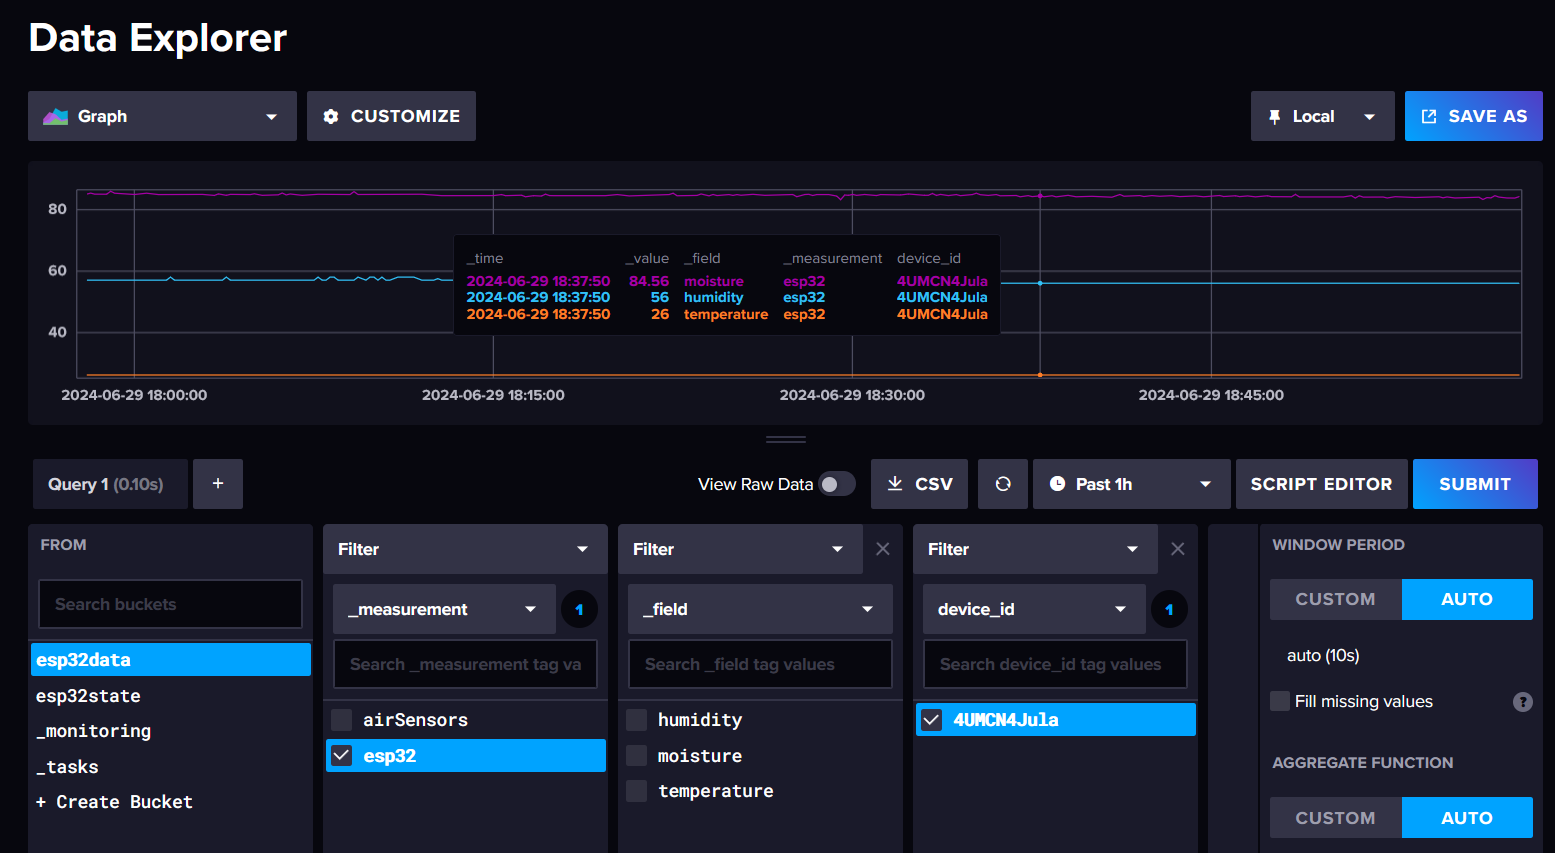
\includegraphics[scale=0.4]{imgs/influxdb}
	\caption{Sučelje za pregled podataka u bazi InfluxDB}
	\label{fig:influxdb}
\end{figure}

Kako je ranije spomenuto, podaci se moraju obraditi Lambda funkcijom kako bi bili pohranjeni u bazu podataka. Stoga je kreirana Lambda funkcija \textit{ESP32Lambda} koja podatke pretvara u format linijskog protokola te ih šalje u InfluxDB. Ova funkcija pokrenuta je pri događaju \engl{event-driven}, što znači da se svakim dolaskom poruka na pretplaćene teme ova funkcija pokrene. AWS podržava brojne programske jezike putem izvršnih okolina u kojima su integrirane značajke potrebne za izvršavanje funkcije u željenom programskom jeziku. Odabir izvršne okoline za sobom povlači i operacijski sustav na kojem se funkcija izvršava. Ova je funkcija napisana u programskom jeziku Python zbog jednostavnosti i razumljivosti programskog koda. Funkcija je naziva \lstinline[language=python]|lambda_handler| koja predstavlja ulaznu točku \engl{entrypoint} za izvršavanje same funkcije. Iako se mogu napisati i pomoćne funkcije, ova je funkcija ključna za izvršavanje skripte. Sastoji se od dva parametra koje joj prosljeđuje proces zaslužan za pokretanje same funkcije, a to su događaj i kontekst. Događaj je zapravo ulazni podatak primljen putem MQTT veze, a objekt konteksta pruža metode i svojstva koja daju informacije o pozivu, samoj funkciji i okolini izvođenja. Funkcija također može koristiti varijable okoline \engl{environment variables} koje se postavljaju odvojeno od samog koda. Postavljanjem varijabli jednostavno se odvajaju tajni parametri od same funkcije. Budući da funkcija zahtijeva stvaranje API poziva prema bazi kako bi zapisala podatke, potrebno je koristiti vanjske biblioteke za kreiranje HTTP zahtjeva. Izvršna okolina Python koda sama po sebi ne pruža tu biblioteku, no moguće je stvoriti dodatan sloj nad Lambda funkcijom koja će sadržavati potreban paket. Slojevi su mehanizam koji omogućavaju dijeljenje i ponovno korištenje zajedničkog koda i resursa između više Lambda funkcija. Omogućava izolaciju dijelova koda, kreiranje i dijeljene biblioteka ili drugih resursa bez potrebe za mijenjanjem postojeće implementacije. Moguće je koristiti slojeve koje nudi AWS, odabrati vanjski sloj koji su kreirali drugi korisnici platforme, ili pak kreirati vlastiti. U razvijenom je sustavu korištena druga opcija, odnosno sloj koji integrira biblioteku \textit{Requests} za kreiranje API poziva. 

Kreirana Lambda funkcija nalazi se u sljedećem programskom isječku. URL baze podataka, oganizacija te kanta za pohranu podataka dohvaćaju se iz varijabli okoline. Isto tako, kako bi funkcija uopće mogla pristupiti bazi, potrebno je generirati token u bazi koji omogućava pisanje u željenu kantu. Generirani je token također zapisan u varijable okoline. Preciznost vremenske oznake postavljena je na milisekunde budući da podaci s uređaja ESP32-C3 dolaze u takvom formatu. Iz funkcije je vidljivo čitanje vrijednosti, stvaranje podatka u formatu linijskog protokola, slanje POST zahtjeva i čekanje na odgovor. 

\begin{lstlisting}[caption={Lambda funkcija za slanje podataka u InfluxDB}, language={python}]
import json
import requests
import time
import os

BUCKET = os.getenv('BUCKET')
ORG = os.getenv('ORG')
INFLUXDB_URL = os.getenv('INFLUXDB_URL')
TOKEN = os.getenv('TOKEN')

def lambda_handler(event, context):
	try:
		measurement = 'esp32'
		timestamp = event["timestamp"]
		device_id = event["device_id"]
		event_data = event["data"]
		fields = ",".join([f"{key}={value}" for key, value in event_data.items() if key != "timestamp" and key != "device_id"])
		data = f"{measurement},device_id={device_id} {fields} {timestamp}"
		print(data)
		headers = {
			'Authorization': f'Token {TOKEN}',
			'Content-Type': 'text/plain'
		}
		params = {
			'org': ORG,
			'bucket': BUCKET,
			'precision': 'ms'
		}
		response = requests.post(
			INFLUXDB_URL,
			headers=headers,
			data=data,
			params=params
		)
		response.raise_for_status()
		print("Data sent to InfluxDB successfully")
	except Exception as e:
		print("Error:", e)
	
	return {
		'statusCode': 200,
		'body': json.dumps('Data processed and sent to InfluxDB')
	}
\end{lstlisting}

\subsection{Sjena uređaja}

Za ažuriranje sjene uređaja u AWS-u nije potrebna nikakva dodatna konfiguracija. Jedini je uvjet da stvar za koju je uređaj vezan postoji, no to je svakako osigurano registracijom na platformu. Uređaj kreira prvotnu klasičnu sjenu uređaja i ažurira je svakom iteracijom programa. Druge aplikacije mogu dohvatiti podatke o sjeni uređaja pretplatom na njegove teme. Prefiks za sve teme jest \lstinline|$aws/things/{thingName}/shadow|. Budući da pregled sjene uređaja u AWS-u sam po sebi nije osobito koristan, po uzoru na proces pohrane senzorskih očitanja, kreirana je ruta koja poruke dospjele na temu ažuriranja sjene prosljeđuje Lambda funkciji, koja pak obrađuje podatke i sprema ih u postojeću bazu InfluxDB. Kreiran je SQL upit koja sve poruke dospjele na temu uspješnog ažuriranja, odnosno poruke prijavljenog stanja, prosljeđuje posebnoj funkciji. 

\begin{lstlisting}[caption={SQL upit rute za sjene uređaja}, language=sql]
	SELECT * FROM '$aws/things/+/shadow/update/accepted'
\end{lstlisting}

Iako sami uređaji u prijavljenom stanju ne postavljaju serijski broj na temelju kojeg bi se izvorišni uređaji mogli razlučiti, svaka poruka sadrži ranije opisani klijentski identifikator na temelju kojeg se kasnije grupiraju podaci. Poruka u formatu JSON koja se rutom proslijedi Lambda funkciji nalazi se u sljedećem programskom isječku. 

\begin{lstlisting}[caption={Poruka ažurirane sjene}, language=json]
{
	"state": {
		"reported": {
			"color": "WHITE"
		}
	},
	"metadata": {
		"reported": {
			"color": {
				"timestamp": 1719764472
			}
		}
	},
	"version": 15299,
	"timestamp": 1719764472,
	"clientToken": "deviceNumber123"
}
\end{lstlisting}

Lambda funkcija sjene uređaja \textit{ESP32ShadowLambda} gotovo je identična funkciji za pohranu podataka, s manjim izmjenama dohvaćanja identifikatora uređaja i promjene vremenske oznake. Biblioteka razvojnog sustava za sjenu uređaja automatski pridjeljuje vremensku oznaku u obliku sekunde, dok API prihvaća podatke na razini milisekunde. Kreirana je nova kanta \textit{esp32state} u bazi InfluxDB koja služi za pohranu stanja sjene. Generiran je i odgovarajući token pisanja u novu kantu, i shodno tome stvorene su nove varijable okoline. Ova se funkcija također bazira na dodatnom sloju koji sadrži paket \textit{Requests} programskog jezika Python za komunikaciju putem API-ja. Isto tako, napravljena je provjera postoji li polje \textit{desired} u JSON objektu, za slučaj da se na temi nađe poruka željenog stanja koja se ne sprema u bazu. Pohrana je namijenjena samo stvarnim ažuriranjima koji dolaze iz poruka prijavljenog stanja.

\begin{lstlisting}[caption={Lambda funkcija za preusmjeravanje poruka sjene uređaja}, language=python]
import json
import requests
import time
import os

BUCKET = os.getenv('BUCKET')
ORG = os.getenv('ORG')
INFLUXDB_URL = os.getenv('INFLUXDB_URL')
TOKEN = os.getenv('TOKEN')

def lambda_handler(event, context):
	if "reported" not in event["state"].keys():
		print("Desired event, skip storing")
	return
	
	try:
		measurement = 'esp32'
		timestamp = event["timestamp"]
		current_state = event["state"]["reported"]
		device_id = event["clientToken"]
		fields = ",".join([f"{key}=\"{value}\"" for key, value in current_state.items() if key != "timestamp" and key != "clientToken"])
		data = f"{measurement},device_id={device_id} {fields} {timestamp * 1000}"
		headers = {
			'Authorization': f'Token {TOKEN}',
			'Content-Type': 'text/plain'
		}
		params = {
			'org': ORG,
			'bucket': BUCKET,
			'precision': 'ms'
		}
		response = requests.post(
			INFLUXDB_URL,
			headers=headers,
			data=data,
			params=params
		)
		response.raise_for_status()
		print("Data sent to InfluxDB successfully")
	except Exception as e:
		print("Error:", e)
	
	return {
		'statusCode': 200,
		'body': json.dumps('Data processed and sent to InfluxDB')
	}
\end{lstlisting}

Slika \ref{fig:influxdb_state} prikazuje podatke sjene uređaja u sučelju baze InfluxDB. Vidljive su promjene stanja kroz vrijeme, odnosno različite vrijednosti boje LED diode koje je uređaj prijavio. 

\begin{figure}[ht]
	\centering
	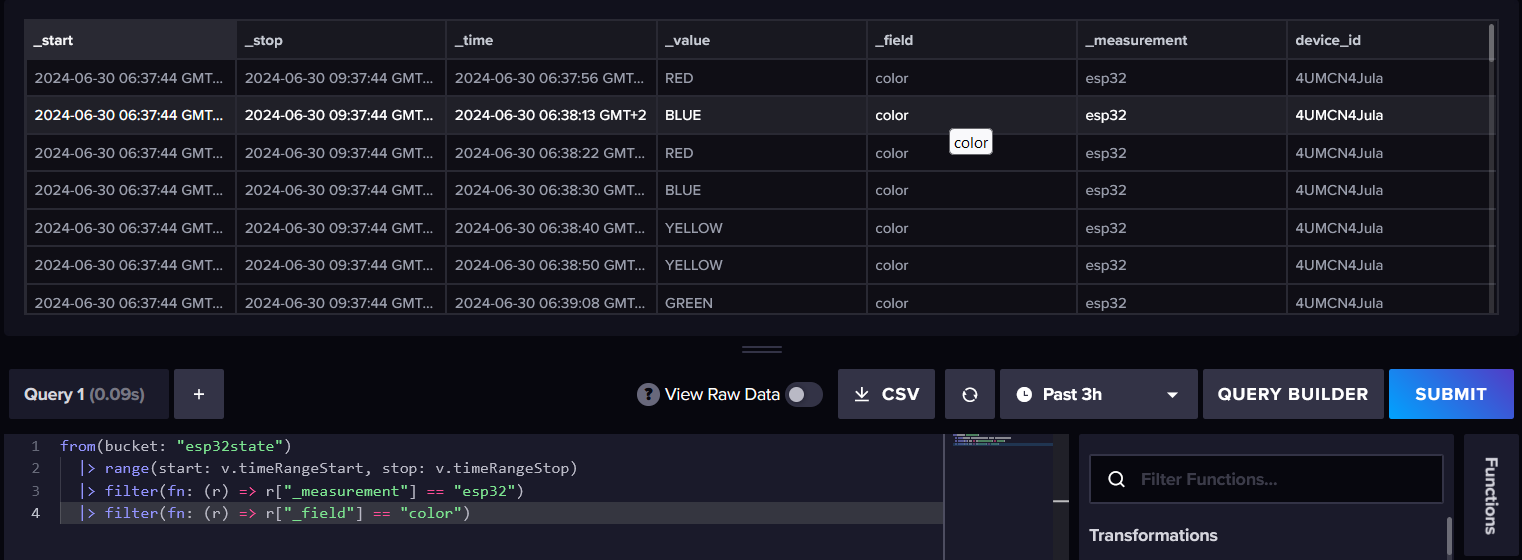
\includegraphics[scale=0.4]{imgs/influxdb_state}
	\caption{Sučelje za pregled stanja uređaja u bazi InfluxDB}
	\label{fig:influxdb_state}
\end{figure}

\subsection{Ažuriranje softvera}
